%% main.tex -- CALE-AI @ AAAI-27 (Evaluating AI Interventions: Causal and Longitudinal Human Effects).
%% Full Research Paper, <= 8 pages EXCLUDING references. AAAI-27 Author Kit, anonymous mode.
%% Conventions: one sentence per line. Every result is \RES{key} from results_macros.tex. Regenerate from the repo root:
%%   .venv/bin/python paper/caleai/caleai_evidence.py
%%   .venv/bin/python paper/caleai/make_macros.py
%%   .venv/bin/python paper/caleai/figs/make_caleai_figs.py
%% Never type a result by hand. Typed design constants (four models, resample counts, seeds, pass lines, power assumptions) are labelled.
%%
%% ======================= SLOTS (A) and (B) FILLED in burn round 1 =======================
%% (A) \slotAuditAbs / \slotAuditBody: the 120-text audit (Part 17) fell under the frozen rule's NONE branch (CI includes 0); numbers are macros from analysis/repair_audit_v2.
%% (B) \slotIntent: writer-intent check (Part 18), macros from analysis/intent_check and analysis/whole_message; full text in Sec. 6.5.
%% Always keep: "the audit can detect a gap of about \RES{dz_mde} points, so no detectable cost is not evidence of no cost".
%%
%% (C) \slotBaseline (Sec. 4 and Sec. 6.1, marked "% BASELINE"): the no-feedback resample baseline (same monitor, regenerate up to two times, no feedback turn). Fill from its analysis file via a macro. Patterns:
%%   FEEDBACK HELPS: "Regeneration without the feedback message repaired X% of strict failures against Y% with it (increment G points [LO, HI]), so the feedback message, not extra draws, earns the increment."
%%   NO DIFFERENCE:  "Regeneration without the feedback message repaired X% against Y% (increment G [LO, HI], including zero): extra draws explain the increment, and the guard's credit shrinks to detection plus resampling."
%%
%% (D) \slotLegend (Sec. 5, cue probe; marked "% LEGEND_TEST"): the three-arm test of whether the prompt's cue legend alone shifts the bare-keyword default. Patterns:
%%   LEGEND MATTERS: "Adding the cue legend to a prompt with no cue changed affirmative output from X% to Y% (gap G [LO, HI]), so the default findings are partly a prompt effect."
%%   NO EFFECT:      "The cue legend alone moved affirmative output by G points [LO, HI], including zero, so the default is not a legend artifact."
%% =========================================================================================
\documentclass[letterpaper]{article} % DO NOT CHANGE THIS
\ifdefined\XeTeXversion% LOCAL PREVIEW ONLY. aaai2027.sty stops on any engine other than pdfTeX (\RequirePDFTeX). The project's
% compiler is Tectonic (XeTeX), so main.tex inputs this shim only when \XeTeXversion is defined. It disables the
% engine guard and changes nothing else. FINAL SUBMISSION: compile with pdflatex (e.g. Overleaf), where the shim
% is skipped automatically, and re-check the page count.
\RequirePackage{iftex}
\let\RequirePDFTeX\relax
\fi % local Tectonic preview only; inert under pdflatex
\usepackage[submission]{aaai2027}  % DO NOT CHANGE THIS
\usepackage[hyphens]{url}  % DO NOT CHANGE THIS
\usepackage{graphicx} % DO NOT CHANGE THIS
\urlstyle{rm} % DO NOT CHANGE THIS
\def\UrlFont{\rm}  % DO NOT CHANGE THIS
\usepackage{natbib}  % DO NOT CHANGE THIS AND DO NOT ADD ANY OPTIONS TO IT
\usepackage{caption} % DO NOT CHANGE THIS AND DO NOT ADD ANY OPTIONS TO IT
\frenchspacing  % DO NOT CHANGE THIS
\usepackage{booktabs}
\usepackage{xcolor}
\usepackage{amsmath}
\usepackage{array}
\usepackage{multirow}
\pdfinfo{
/TemplateVersion (2027.1)
}
\setcounter{secnumdepth}{2}
\graphicspath{{figs/}}

%% ---------- results macros ----------
\makeatletter
\newcommand{\resdef}[2]{\expandafter\def\csname RES@#1\endcsname{#2}}
\newcommand{\RES}[1]{\ifcsname RES@#1\endcsname\csname RES@#1\endcsname\else\RESmissing{#1}\fi}
\newcommand{\RESmissing}[1]{\textcolor{red}{\textbf{\texttt{[\detokenize{#1}]}}}}
\newcommand{\IfRES}[3]{\ifcsname RES@#1\endcsname#2\else#3\fi}
\newcommand{\inputrows}[1]{\@@input #1 } % primitive (expandable) input: generated rows inside a tabular
\makeatother
% AUTO-GENERATED by make_macros.py from evidence.json + analysis/evidence_c3/current.json -- do not edit by hand.
\resdef{app_chip1_avail}{1,904}
\resdef{app_chip1_d}{25.76}
\resdef{app_chip1_d_hi}{27.88}
\resdef{app_chip1_d_lo}{23.69}
\resdef{app_chip1_ncl}{210}
\resdef{app_chip1_p0}{12.09}
\resdef{app_chip1_p0_hi}{14.48}
\resdef{app_chip1_p0_lo}{9.75}
\resdef{app_chip1_p0c}{12.1}
\resdef{app_chip1_p0c_k}{223}
\resdef{app_chip1_p0c_n}{1,844}
\resdef{app_chip1_p2}{38.67}
\resdef{app_chip1_p2_hi}{41.89}
\resdef{app_chip1_p2_lo}{35.47}
\resdef{app_chip1_p2c}{38.7}
\resdef{app_chip1_p2c_k}{713}
\resdef{app_chip1_p2c_n}{1,844}
\resdef{app_chip1_s3}{12.91}
\resdef{app_chip1_s3_hi}{15.60}
\resdef{app_chip1_s3_lo}{10.36}
\resdef{app_chip1_s3c}{12.9}
\resdef{app_chip1_s3c_k}{238}
\resdef{app_chip1_s3c_n}{1,844}
\resdef{app_chipall_avail}{1,904}
\resdef{app_chipall_d}{22.98}
\resdef{app_chipall_d_hi}{24.64}
\resdef{app_chipall_d_lo}{21.38}
\resdef{app_chipall_ncl}{210}
\resdef{app_chipall_p0}{13.21}
\resdef{app_chipall_p0_hi}{15.55}
\resdef{app_chipall_p0_lo}{10.95}
\resdef{app_chipall_p0c}{13.2}
\resdef{app_chipall_p0c_k}{245}
\resdef{app_chipall_p0c_n}{1,854}
\resdef{app_chipall_p2}{37.43}
\resdef{app_chipall_p2_hi}{40.07}
\resdef{app_chipall_p2_lo}{34.93}
\resdef{app_chipall_p2c}{37.4}
\resdef{app_chipall_p2c_k}{694}
\resdef{app_chipall_p2c_n}{1,854}
\resdef{app_chipall_s3}{14.46}
\resdef{app_chipall_s3_hi}{16.88}
\resdef{app_chipall_s3_lo}{12.13}
\resdef{app_chipall_s3c}{14.5}
\resdef{app_chipall_s3c_k}{268}
\resdef{app_chipall_s3c_n}{1,854}
\resdef{app_ex_d}{2.97}
\resdef{app_ex_d_hi}{4.54}
\resdef{app_ex_d_lo}{1.55}
\resdef{app_ex_ncl}{79}
\resdef{app_ex_p0}{0.16}
\resdef{app_ex_p0_hi}{0.48}
\resdef{app_ex_p0_k}{1}
\resdef{app_ex_p0_lo}{0.00}
\resdef{app_ex_p0_n}{639}
\resdef{app_ex_p2}{3.29}
\resdef{app_ex_p2_hi}{4.85}
\resdef{app_ex_p2_k}{21}
\resdef{app_ex_p2_lo}{1.88}
\resdef{app_ex_p2_n}{639}
\resdef{app_ex_s3}{0.31}
\resdef{app_ex_s3_hi}{0.79}
\resdef{app_ex_s3_k}{2}
\resdef{app_ex_s3_lo}{0.00}
\resdef{app_ex_s3_n}{639}
\resdef{app_full_avail}{1,904}
\resdef{app_full_d}{60.05}
\resdef{app_full_d_hi}{62.70}
\resdef{app_full_d_lo}{57.31}
\resdef{app_full_d_noearly}{59.92}
\resdef{app_full_d_noearly_hi}{62.64}
\resdef{app_full_d_noearly_lo}{57.13}
\resdef{app_full_ncl}{210}
\resdef{app_full_p0}{2.05}
\resdef{app_full_p0_hi}{2.76}
\resdef{app_full_p0_lo}{1.41}
\resdef{app_full_p0c}{2.1}
\resdef{app_full_p0c_k}{38}
\resdef{app_full_p0c_n}{1,850}
\resdef{app_full_p2}{62.76}
\resdef{app_full_p2_hi}{65.53}
\resdef{app_full_p2_lo}{59.89}
\resdef{app_full_p2c}{62.8}
\resdef{app_full_p2c_k}{1,161}
\resdef{app_full_p2c_n}{1,850}
\resdef{app_full_s3}{2.70}
\resdef{app_full_s3_hi}{3.54}
\resdef{app_full_s3_lo}{1.94}
\resdef{app_full_s3c}{2.7}
\resdef{app_full_s3c_k}{50}
\resdef{app_full_s3c_n}{1,850}
\resdef{app_ready}{1}
\resdef{c3_app_first_p0}{2.05}
\resdef{c3_app_first_p0_clusters}{210}
\resdef{c3_app_first_p0_hi}{2.76}
\resdef{c3_app_first_p0_k}{38}
\resdef{c3_app_first_p0_lo}{1.41}
\resdef{c3_app_first_p0_n}{1,850}
\resdef{c3_app_first_p2}{29.14}
\resdef{c3_app_first_p2_clusters}{210}
\resdef{c3_app_first_p2_hi}{31.37}
\resdef{c3_app_first_p2_k}{539}
\resdef{c3_app_first_p2_lo}{26.92}
\resdef{c3_app_first_p2_minus_p0}{27.08}
\resdef{c3_app_first_p2_minus_p0_clusters}{210}
\resdef{c3_app_first_p2_minus_p0_hi}{29.19}
\resdef{c3_app_first_p2_minus_p0_lo}{25.03}
\resdef{c3_app_first_p2_minus_s3}{27.08}
\resdef{c3_app_first_p2_minus_s3_clusters}{210}
\resdef{c3_app_first_p2_minus_s3_hi}{29.22}
\resdef{c3_app_first_p2_minus_s3_lo}{24.97}
\resdef{c3_app_first_p2_n}{1,850}
\resdef{c3_app_first_s3}{2.05}
\resdef{c3_app_first_s3_clusters}{210}
\resdef{c3_app_first_s3_hi}{2.79}
\resdef{c3_app_first_s3_k}{38}
\resdef{c3_app_first_s3_lo}{1.39}
\resdef{c3_app_first_s3_n}{1,850}
\resdef{c3_guard_g1_only}{31}
\resdef{c3_guard_increment}{2.08}
\resdef{c3_guard_increment_clusters}{58}
\resdef{c3_guard_increment_hi}{3.16}
\resdef{c3_guard_increment_lo}{1.15}
\resdef{c3_guard_increment_n}{1,392}
\resdef{c3_guard_pass_g1}{1,375}
\resdef{c3_guard_pass_g1s}{1,346}
\resdef{c3_guard_pass_p0}{1,312}
\resdef{c3_guard_strip_only}{2}
\resdef{c_act_chip1}{81.2}
\resdef{c_act_noncrit}{43.8}
\resdef{c_agt_chip1}{100.0}
\resdef{c_agt_noncrit}{47.5}
\resdef{c_bare}{38.8}
\resdef{c_bare_hi}{43.3}
\resdef{c_bare_k}{180}
\resdef{c_bare_lo}{33.8}
\resdef{c_bare_n}{464}
\resdef{c_cer_chip1}{98.8}
\resdef{c_cer_noncrit}{48.8}
\resdef{c_chip1}{94.8}
\resdef{c_chip1_gemma}{93.1}
\resdef{c_chip1_hi}{97.6}
\resdef{c_chip1_k}{440}
\resdef{c_chip1_llama}{94.0}
\resdef{c_chip1_lo}{91.4}
\resdef{c_chip1_n}{464}
\resdef{c_chip1_qwen}{95.7}
\resdef{c_chip1_terra}{96.6}
\resdef{c_chip1contra}{0.0}
\resdef{c_chip1contra_hi}{0.0}
\resdef{c_chip1contra_k}{0}
\resdef{c_chip1contra_lo}{0.0}
\resdef{c_chip1contra_n}{464}
\resdef{c_chip1poladd}{3.2}
\resdef{c_chip1poladd_hi}{5.0}
\resdef{c_chip1poladd_k}{15}
\resdef{c_chip1poladd_lo}{1.5}
\resdef{c_chip1poladd_n}{464}
\resdef{c_chipall}{95.9}
\resdef{c_chipall_hi}{97.4}
\resdef{c_chipall_k}{445}
\resdef{c_chipall_lo}{94.2}
\resdef{c_chipall_n}{464}
\resdef{c_d}{53.0}
\resdef{c_d_hi}{58.2}
\resdef{c_d_k}{246}
\resdef{c_d_lo}{47.8}
\resdef{c_d_n}{464}
\resdef{c_full}{97.4}
\resdef{c_full_hi}{99.1}
\resdef{c_full_k}{452}
\resdef{c_full_lo}{95.0}
\resdef{c_full_n}{464}
\resdef{c_lostwithchip}{3.6}
\resdef{c_lostwithchip_hi}{6.9}
\resdef{c_lostwithchip_k}{7}
\resdef{c_lostwithchip_lo}{1.0}
\resdef{c_lostwithchip_n}{194}
\resdef{c_misspersists}{7.4}
\resdef{c_misspersists_hi}{12.6}
\resdef{c_misspersists_k}{21}
\resdef{c_misspersists_lo}{3.0}
\resdef{c_misspersists_n}{284}
\resdef{c_n}{464}
\resdef{c_nchips}{3.1}
\resdef{c_noncrit}{41.8}
\resdef{c_noncrit_gemma}{38.8}
\resdef{c_noncrit_hi}{45.9}
\resdef{c_noncrit_k}{194}
\resdef{c_noncrit_llama}{44.0}
\resdef{c_noncrit_lo}{37.1}
\resdef{c_noncrit_n}{464}
\resdef{c_noncrit_qwen}{42.2}
\resdef{c_noncrit_terra}{42.2}
\resdef{c_noncritpoladd}{9.1}
\resdef{c_noncritpoladd_hi}{13.1}
\resdef{c_noncritpoladd_k}{42}
\resdef{c_noncritpoladd_lo}{5.6}
\resdef{c_noncritpoladd_n}{464}
\resdef{c_pol_chip1}{100.0}
\resdef{c_pol_noncrit}{50.0}
\resdef{c_pz_chip1}{90.0}
\resdef{c_pz_noncrit}{50.0}
\resdef{c_ratio}{97.3}
\resdef{c_tq_chip1}{96.2}
\resdef{c_tq_noncrit}{11.2}
\resdef{copy_k}{116}
\resdef{copy_n}{116}
\resdef{g_amb_fix}{100.0}
\resdef{g_amb_fix_k}{86}
\resdef{g_amb_fix_n}{86}
\resdef{g_ask}{6.3}
\resdef{g_ask_k}{4}
\resdef{g_ask_n}{63}
\resdef{g_bad_all}{166}
\resdef{g_broken}{0.0}
\resdef{g_broken_cue}{0.0}
\resdef{g_broken_cue_k}{0}
\resdef{g_broken_cue_n}{1,312}
\resdef{g_broken_hi}{0.0}
\resdef{g_broken_lo}{0.0}
\resdef{g_broken_n}{2,154}
\resdef{g_calls}{0.104}
\resdef{g_calls_flag}{1.23}
\resdef{g_calls_incl}{0.112}
\resdef{g_check_ms}{2.3}
\resdef{g_cm_g1}{99.2}
\resdef{g_cm_g1_hi}{99.8}
\resdef{g_cm_g1_lo}{98.5}
\resdef{g_cm_g1_n}{1,392}
\resdef{g_cm_g1s}{97.9}
\resdef{g_cm_g1s_hi}{99.1}
\resdef{g_cm_g1s_lo}{96.5}
\resdef{g_cm_g1s_n}{1,392}
\resdef{g_cm_p0}{96.0}
\resdef{g_cm_p0_hi}{97.7}
\resdef{g_cm_p0_lo}{94.2}
\resdef{g_cm_p0_n}{1,392}
\resdef{g_cmp_n}{1,392}
\resdef{g_cpx_g1}{98.85}
\resdef{g_cpx_g1_hi}{99.50}
\resdef{g_cpx_g1_lo}{98.13}
\resdef{g_cpx_g1_n}{1,392}
\resdef{g_cpx_g1s}{96.77}
\resdef{g_cpx_g1s_hi}{98.06}
\resdef{g_cpx_g1s_lo}{95.26}
\resdef{g_cpx_g1s_n}{1,392}
\resdef{g_cpx_p0}{94.68}
\resdef{g_cpx_p0_hi}{96.70}
\resdef{g_cpx_p0_lo}{92.39}
\resdef{g_cpx_p0_n}{1,392}
\resdef{g_ct_g1}{0.4}
\resdef{g_ct_g1_hi}{0.8}
\resdef{g_ct_g1_lo}{0.1}
\resdef{g_ct_g1_n}{1,392}
\resdef{g_ct_g1s}{1.3}
\resdef{g_ct_g1s_hi}{2.0}
\resdef{g_ct_g1s_lo}{0.6}
\resdef{g_ct_g1s_n}{1,392}
\resdef{g_ct_p0}{1.6}
\resdef{g_ct_p0_hi}{2.4}
\resdef{g_ct_p0_lo}{0.9}
\resdef{g_ct_p0_n}{1,392}
\resdef{g_fix}{78.8}
\resdef{g_fix_all}{89.8}
\resdef{g_fix_all_hi}{95.0}
\resdef{g_fix_all_lo}{83.9}
\resdef{g_fix_all_n}{166}
\resdef{g_fix_fam}{26}
\resdef{g_fix_gemma}{87.9}
\resdef{g_fix_gemma_k}{29}
\resdef{g_fix_gemma_n}{33}
\resdef{g_fix_hi}{88.9}
\resdef{g_fix_incl}{72.0}
\resdef{g_fix_incl_hi}{84.2}
\resdef{g_fix_incl_lo}{59.6}
\resdef{g_fix_incl_n}{93}
\resdef{g_fix_llama}{76.9}
\resdef{g_fix_llama_k}{20}
\resdef{g_fix_llama_n}{26}
\resdef{g_fix_lo}{68.4}
\resdef{g_fix_n}{80}
\resdef{g_fix_qwen}{53.8}
\resdef{g_fix_qwen_k}{7}
\resdef{g_fix_qwen_n}{13}
\resdef{g_fix_terra}{87.5}
\resdef{g_fix_terra_k}{7}
\resdef{g_fix_terra_n}{8}
\resdef{g_fixc}{78.8}
\resdef{g_fixc_incl}{72.0}
\resdef{g_fixc_incl_k}{67}
\resdef{g_fixc_incl_n}{93}
\resdef{g_fixc_k}{63}
\resdef{g_fixc_n}{80}
\resdef{g_fixs}{42.5}
\resdef{g_fixs_hi}{54.4}
\resdef{g_fixs_lo}{28.8}
\resdef{g_fixs_n}{80}
\resdef{g_fixsc}{42.5}
\resdef{g_fixsc_k}{34}
\resdef{g_fixsc_n}{80}
\resdef{g_flagged}{8.5}
\resdef{g_flagged_k}{157}
\resdef{g_flagged_n}{1,856}
\resdef{g_lat}{0.17}
\resdef{g_lat_flag_med}{1.59}
\resdef{g_oc_all}{2.3}
\resdef{g_oc_all_hi}{3.6}
\resdef{g_oc_all_lo}{1.1}
\resdef{g_oc_all_n}{2,154}
\resdef{g_oc_amb}{4.2}
\resdef{g_oc_amb_hi}{7.2}
\resdef{g_oc_amb_lo}{1.5}
\resdef{g_oc_amb_n}{842}
\resdef{g_oc_cue}{1.1}
\resdef{g_oc_cue_k}{14}
\resdef{g_oc_cue_n}{1,312}
\resdef{g_occ_all}{2.3}
\resdef{g_occ_all_k}{49}
\resdef{g_occ_all_n}{2,154}
\resdef{g_occue_gemma}{1.0}
\resdef{g_occue_gemma_k}{3}
\resdef{g_occue_gemma_n}{315}
\resdef{g_occue_llama}{1.6}
\resdef{g_occue_llama_k}{5}
\resdef{g_occue_llama_n}{322}
\resdef{g_occue_qwen}{0.9}
\resdef{g_occue_qwen_k}{3}
\resdef{g_occue_qwen_n}{335}
\resdef{g_occue_terra}{0.9}
\resdef{g_occue_terra_k}{3}
\resdef{g_occue_terra_n}{340}
\resdef{g_ocs_all}{1.6}
\resdef{g_ocs_all_hi}{2.7}
\resdef{g_ocs_all_lo}{0.6}
\resdef{g_ocs_all_n}{2,154}
\resdef{g_ocsc_all}{1.6}
\resdef{g_ocsc_all_k}{34}
\resdef{g_ocsc_all_n}{2,154}
\resdef{g_pa_g1}{0.1}
\resdef{g_pa_g1_hi}{0.4}
\resdef{g_pa_g1_lo}{0.0}
\resdef{g_pa_g1_n}{1,392}
\resdef{g_pa_g1s}{0.1}
\resdef{g_pa_g1s_hi}{0.4}
\resdef{g_pa_g1s_lo}{0.0}
\resdef{g_pa_g1s_n}{1,392}
\resdef{g_pa_p0}{2.7}
\resdef{g_pa_p0_hi}{4.0}
\resdef{g_pa_p0_lo}{1.4}
\resdef{g_pa_p0_n}{1,392}
\resdef{g_res}{1.2}
\resdef{g_res_act}{70.6}
\resdef{g_res_act_k}{12}
\resdef{g_res_act_n}{17}
\resdef{g_res_flag}{82.4}
\resdef{g_res_flag_k}{14}
\resdef{g_res_flag_n}{17}
\resdef{g_res_hi}{2.1}
\resdef{g_res_k}{17}
\resdef{g_res_lo}{0.5}
\resdef{g_res_n}{1,392}
\resdef{g_s_gain}{2.44}
\resdef{g_sp0_gemma}{90.5}
\resdef{g_sp0_llama}{92.5}
\resdef{g_sp0_qwen}{96.3}
\resdef{g_sp0_terra}{97.7}
\resdef{g_sp1_gemma}{98.9}
\resdef{g_sp1_llama}{98.3}
\resdef{g_sp1_qwen}{98.3}
\resdef{g_sp1_terra}{99.7}
\resdef{g_sp_g1}{98.8}
\resdef{g_sp_g1_hi}{99.5}
\resdef{g_sp_g1_lo}{97.9}
\resdef{g_sp_g1_n}{1,392}
\resdef{g_sp_g1s}{96.7}
\resdef{g_sp_g1s_hi}{98.1}
\resdef{g_sp_g1s_lo}{95.2}
\resdef{g_sp_g1s_n}{1,392}
\resdef{g_sp_gain}{4.53}
\resdef{g_sp_p0}{94.3}
\resdef{g_sp_p0_hi}{96.3}
\resdef{g_sp_p0_lo}{91.9}
\resdef{g_sp_p0_n}{1,392}
\resdef{g_spc_g1}{1,375}
\resdef{g_spc_g1s}{1,346}
\resdef{g_spc_p0}{1,312}
\resdef{g_spx_g1}{98.78}
\resdef{g_spx_g1_hi}{99.50}
\resdef{g_spx_g1_lo}{97.92}
\resdef{g_spx_g1_n}{1,392}
\resdef{g_spx_g1s}{96.70}
\resdef{g_spx_g1s_hi}{98.06}
\resdef{g_spx_g1s_lo}{95.18}
\resdef{g_spx_g1s_n}{1,392}
\resdef{g_spx_p0}{94.25}
\resdef{g_spx_p0_hi}{96.34}
\resdef{g_spx_p0_lo}{91.88}
\resdef{g_spx_p0_n}{1,392}
\resdef{g_unfixed}{21.2}
\resdef{g_unfixed_k}{17}
\resdef{g_unfixed_n}{80}
\resdef{gt_F}{508}
\resdef{gt_calls}{0.41}
\resdef{gt_calls_flag}{1.51}
\resdef{gt_cc_g1}{1.87}
\resdef{gt_cc_g1_hi}{2.64}
\resdef{gt_cc_g1_k}{26}
\resdef{gt_cc_g1_lo}{1.16}
\resdef{gt_cc_g1_n}{1,394}
\resdef{gt_cc_g1s}{0.00}
\resdef{gt_cc_g1s_hi}{0.00}
\resdef{gt_cc_g1s_k}{0}
\resdef{gt_cc_g1s_lo}{0.00}
\resdef{gt_cc_g1s_n}{1,394}
\resdef{gt_cc_le10}{passes}
\resdef{gt_cmp_joint}{6.36}
\resdef{gt_cmp_joint_g1only}{123}
\resdef{gt_cmp_joint_g1sonly}{4}
\resdef{gt_cmp_joint_hi}{7.48}
\resdef{gt_cmp_joint_k}{119}
\resdef{gt_cmp_joint_lo}{5.29}
\resdef{gt_cmp_joint_n}{1,872}
\resdef{gt_cmp_strict}{6.14}
\resdef{gt_cmp_strict_g1only}{128}
\resdef{gt_cmp_strict_g1sonly}{13}
\resdef{gt_cmp_strict_hi}{7.43}
\resdef{gt_cmp_strict_k}{115}
\resdef{gt_cmp_strict_lo}{4.91}
\resdef{gt_cmp_strict_n}{1,872}
\resdef{gt_crit_changedcorrectle10}{passes}
\resdef{gt_crit_completedfulldesign}{passes}
\resdef{gt_crit_positivejointgainlower95gt0}{passes}
\resdef{gt_crit_repairge30}{passes}
\resdef{gt_crit_withinbudget}{passes}
\resdef{gt_ex_cc_model}{Qwen}
\resdef{gt_fam}{78}
\resdef{gt_flagged_g1}{511}
\resdef{gt_flagged_g1s}{511}
\resdef{gt_gen_calls}{766}
\resdef{gt_gen_cap}{2,000}
\resdef{gt_jgain_g1}{9.83}
\resdef{gt_jgain_g1_hi}{11.32}
\resdef{gt_jgain_g1_k}{184}
\resdef{gt_jgain_g1_lo}{8.39}
\resdef{gt_jgain_g1_n}{1,872}
\resdef{gt_jgain_g1s}{3.47}
\resdef{gt_jgain_g1s_hi}{4.22}
\resdef{gt_jgain_g1s_k}{65}
\resdef{gt_jgain_g1s_lo}{2.78}
\resdef{gt_jgain_g1s_n}{1,872}
\resdef{gt_jgain_gemma}{19.02}
\resdef{gt_jgain_gemma_hi}{22.86}
\resdef{gt_jgain_gemma_k}{89}
\resdef{gt_jgain_gemma_lo}{15.38}
\resdef{gt_jgain_gemma_n}{468}
\resdef{gt_jgain_llama}{16.24}
\resdef{gt_jgain_llama_hi}{19.44}
\resdef{gt_jgain_llama_k}{76}
\resdef{gt_jgain_llama_lo}{13.25}
\resdef{gt_jgain_llama_n}{468}
\resdef{gt_jgain_qwen}{3.21}
\resdef{gt_jgain_qwen_hi}{4.70}
\resdef{gt_jgain_qwen_k}{15}
\resdef{gt_jgain_qwen_lo}{1.92}
\resdef{gt_jgain_qwen_n}{468}
\resdef{gt_jgain_terra}{0.85}
\resdef{gt_jgain_terra_hi}{1.71}
\resdef{gt_jgain_terra_k}{4}
\resdef{gt_jgain_terra_lo}{0.21}
\resdef{gt_jgain_terra_n}{468}
\resdef{gt_jp_g1}{88.62}
\resdef{gt_jp_g1_chip1}{81.41}
\resdef{gt_jp_g1_chip1_hi}{84.62}
\resdef{gt_jp_g1_chip1_k}{508}
\resdef{gt_jp_g1_chip1_lo}{78.04}
\resdef{gt_jp_g1_chip1_n}{624}
\resdef{gt_jp_g1_chipall}{85.10}
\resdef{gt_jp_g1_chipall_hi}{88.14}
\resdef{gt_jp_g1_chipall_k}{531}
\resdef{gt_jp_g1_chipall_lo}{81.89}
\resdef{gt_jp_g1_chipall_n}{624}
\resdef{gt_jp_g1_full}{99.36}
\resdef{gt_jp_g1_full_hi}{99.84}
\resdef{gt_jp_g1_full_k}{620}
\resdef{gt_jp_g1_full_lo}{98.72}
\resdef{gt_jp_g1_full_n}{624}
\resdef{gt_jp_g1_hi}{90.38}
\resdef{gt_jp_g1_k}{1,659}
\resdef{gt_jp_g1_lo}{86.91}
\resdef{gt_jp_g1_n}{1,872}
\resdef{gt_jp_g1s}{82.26}
\resdef{gt_jp_g1s_hi}{84.35}
\resdef{gt_jp_g1s_k}{1,540}
\resdef{gt_jp_g1s_lo}{80.29}
\resdef{gt_jp_g1s_n}{1,872}
\resdef{gt_jp_p0}{78.79}
\resdef{gt_jp_p0_chip1}{73.24}
\resdef{gt_jp_p0_chip1_hi}{76.92}
\resdef{gt_jp_p0_chip1_k}{457}
\resdef{gt_jp_p0_chip1_lo}{69.39}
\resdef{gt_jp_p0_chip1_n}{624}
\resdef{gt_jp_p0_chipall}{66.51}
\resdef{gt_jp_p0_chipall_hi}{71.15}
\resdef{gt_jp_p0_chipall_k}{415}
\resdef{gt_jp_p0_chipall_lo}{61.86}
\resdef{gt_jp_p0_chipall_n}{624}
\resdef{gt_jp_p0_full}{96.63}
\resdef{gt_jp_p0_full_hi}{98.08}
\resdef{gt_jp_p0_full_k}{603}
\resdef{gt_jp_p0_full_lo}{94.87}
\resdef{gt_jp_p0_full_n}{624}
\resdef{gt_jp_p0_hi}{81.41}
\resdef{gt_jp_p0_k}{1,475}
\resdef{gt_jp_p0_lo}{76.23}
\resdef{gt_jp_p0_n}{1,872}
\resdef{gt_jrep_g1}{46.35}
\resdef{gt_jrep_g1_hi}{50.86}
\resdef{gt_jrep_g1_k}{184}
\resdef{gt_jrep_g1_lo}{41.96}
\resdef{gt_jrep_g1_n}{397}
\resdef{gt_jrep_g1s}{16.88}
\resdef{gt_jrep_g1s_hi}{18.75}
\resdef{gt_jrep_g1s_k}{67}
\resdef{gt_jrep_g1s_lo}{14.93}
\resdef{gt_jrep_g1s_n}{397}
\resdef{gt_judge_calls}{207}
\resdef{gt_judge_cap}{400}
\resdef{gt_pa_g1}{0.96}
\resdef{gt_pa_g1_hi}{1.50}
\resdef{gt_pa_g1_k}{18}
\resdef{gt_pa_g1_lo}{0.53}
\resdef{gt_pa_g1_n}{1,872}
\resdef{gt_pa_g1s}{0.64}
\resdef{gt_pa_g1s_hi}{1.01}
\resdef{gt_pa_g1s_k}{12}
\resdef{gt_pa_g1s_lo}{0.32}
\resdef{gt_pa_g1s_n}{1,872}
\resdef{gt_pa_p0}{9.08}
\resdef{gt_pa_p0_hi}{10.79}
\resdef{gt_pa_p0_k}{170}
\resdef{gt_pa_p0_lo}{7.43}
\resdef{gt_pa_p0_n}{1,872}
\resdef{gt_pf_g1}{0.00}
\resdef{gt_pf_g1_hi}{0.00}
\resdef{gt_pf_g1_k}{0}
\resdef{gt_pf_g1_lo}{0.00}
\resdef{gt_pf_g1_n}{1,394}
\resdef{gt_pf_g1s}{0.00}
\resdef{gt_pf_g1s_hi}{0.00}
\resdef{gt_pf_g1s_k}{0}
\resdef{gt_pf_g1s_lo}{0.00}
\resdef{gt_pf_g1s_n}{1,394}
\resdef{gt_ready}{1}
\resdef{gt_rep_g1}{52.51}
\resdef{gt_rep_g1_hi}{56.70}
\resdef{gt_rep_g1_k}{251}
\resdef{gt_rep_g1_lo}{48.36}
\resdef{gt_rep_g1_n}{478}
\resdef{gt_rep_g1s}{28.45}
\resdef{gt_rep_g1s_hi}{31.15}
\resdef{gt_rep_g1s_k}{136}
\resdef{gt_rep_g1s_lo}{25.49}
\resdef{gt_rep_g1s_n}{478}
\resdef{gt_rep_ge30}{passes}
\resdef{gt_rep_gemma}{72.32}
\resdef{gt_rep_gemma_hi}{77.46}
\resdef{gt_rep_gemma_k}{128}
\resdef{gt_rep_gemma_lo}{67.22}
\resdef{gt_rep_gemma_n}{177}
\resdef{gt_rep_llama}{54.04}
\resdef{gt_rep_llama_hi}{61.94}
\resdef{gt_rep_llama_k}{87}
\resdef{gt_rep_llama_lo}{46.33}
\resdef{gt_rep_llama_n}{161}
\resdef{gt_rep_qwen}{18.52}
\resdef{gt_rep_qwen_hi}{25.88}
\resdef{gt_rep_qwen_k}{15}
\resdef{gt_rep_qwen_lo}{11.39}
\resdef{gt_rep_qwen_n}{81}
\resdef{gt_rep_terra}{35.59}
\resdef{gt_rep_terra_hi}{49.06}
\resdef{gt_rep_terra_k}{21}
\resdef{gt_rep_terra_lo}{23.81}
\resdef{gt_rep_terra_n}{59}
\resdef{gt_res_g1}{12.13}
\resdef{gt_res_g1_hi}{14.00}
\resdef{gt_res_g1_k}{227}
\resdef{gt_res_g1_lo}{10.20}
\resdef{gt_res_g1_n}{1,872}
\resdef{gt_res_g1s}{18.27}
\resdef{gt_res_g1s_hi}{20.41}
\resdef{gt_res_g1s_k}{342}
\resdef{gt_res_g1s_lo}{16.08}
\resdef{gt_res_g1s_n}{1,872}
\resdef{gt_resflag_g1_k}{215}
\resdef{gt_resflag_g1_n}{227}
\resdef{gt_resflag_g1s_k}{339}
\resdef{gt_resflag_g1s_n}{342}
\resdef{gt_resid_flag_unique}{226}
\resdef{gt_sgain_g1}{13.41}
\resdef{gt_sgain_g1_hi}{15.44}
\resdef{gt_sgain_g1_k}{251}
\resdef{gt_sgain_g1_lo}{11.38}
\resdef{gt_sgain_g1_n}{1,872}
\resdef{gt_sgain_g1s}{7.26}
\resdef{gt_sgain_g1s_hi}{8.71}
\resdef{gt_sgain_g1s_k}{136}
\resdef{gt_sgain_g1s_lo}{5.88}
\resdef{gt_sgain_g1s_n}{1,872}
\resdef{gt_sp_g1}{87.87}
\resdef{gt_sp_g1_hi}{89.80}
\resdef{gt_sp_g1_k}{1,645}
\resdef{gt_sp_g1_lo}{86.00}
\resdef{gt_sp_g1_n}{1,872}
\resdef{gt_sp_g1s}{81.73}
\resdef{gt_sp_g1s_hi}{83.92}
\resdef{gt_sp_g1s_k}{1,530}
\resdef{gt_sp_g1s_lo}{79.59}
\resdef{gt_sp_g1s_n}{1,872}
\resdef{gt_sp_p0}{74.47}
\resdef{gt_sp_p0_hi}{77.78}
\resdef{gt_sp_p0_k}{1,394}
\resdef{gt_sp_p0_lo}{71.26}
\resdef{gt_sp_p0_n}{1,872}
\resdef{gt_targets}{1,872}
\resdef{gt_unique}{1,848}
\resdef{gt_usable_validated}{no}
\resdef{gt_verdict}{passed}
\resdef{human_act_acc}{96.9}
\resdef{human_act_acc_hi}{98.7}
\resdef{human_act_acc_k}{155}
\resdef{human_act_acc_lo}{92.9}
\resdef{human_act_accw}{97.6}
\resdef{human_act_alpha}{1.00}
\resdef{human_act_alpha_hi}{1.00}
\resdef{human_act_alpha_lo}{1.00}
\resdef{human_act_alpha_n}{98}
\resdef{human_act_chacc}{100.0}
\resdef{human_act_chacc_k}{23}
\resdef{human_act_chn}{23}
\resdef{human_act_gate}{pass}
\resdef{human_act_gkappa}{0.94}
\resdef{human_act_gkappa_hi}{0.99}
\resdef{human_act_gkappa_lo}{0.88}
\resdef{human_act_gn}{118}
\resdef{human_act_kappa}{0.94}
\resdef{human_act_kappa_hi}{0.99}
\resdef{human_act_kappa_lo}{0.89}
\resdef{human_act_kappaw}{0.95}
\resdef{human_act_kappaw_hi}{1.00}
\resdef{human_act_kappaw_lo}{0.88}
\resdef{human_act_n}{160}
\resdef{human_act_nnull}{0}
\resdef{human_act_noconsensus}{0}
\resdef{human_add_acc}{95.1}
\resdef{human_add_acc_hi}{97.6}
\resdef{human_add_acc_k}{137}
\resdef{human_add_acc_lo}{90.3}
\resdef{human_add_accw}{95.9}
\resdef{human_add_alpha}{0.98}
\resdef{human_add_alpha_hi}{1.00}
\resdef{human_add_alpha_lo}{0.92}
\resdef{human_add_alpha_n}{100}
\resdef{human_add_chacc}{100.0}
\resdef{human_add_chacc_k}{24}
\resdef{human_add_chn}{24}
\resdef{human_add_gate}{pass}
\resdef{human_add_gkappa}{0.91}
\resdef{human_add_gkappa_hi}{0.98}
\resdef{human_add_gkappa_lo}{0.81}
\resdef{human_add_gn}{107}
\resdef{human_add_kappa}{0.90}
\resdef{human_add_kappa_hi}{0.96}
\resdef{human_add_kappa_lo}{0.83}
\resdef{human_add_kappaw}{0.91}
\resdef{human_add_kappaw_hi}{0.97}
\resdef{human_add_kappaw_lo}{0.84}
\resdef{human_add_n}{144}
\resdef{human_add_nnull}{18}
\resdef{human_add_noconsensus}{1}
\resdef{human_agt_acc}{95.0}
\resdef{human_agt_acc_hi}{97.4}
\resdef{human_agt_acc_k}{151}
\resdef{human_agt_acc_lo}{90.4}
\resdef{human_agt_accw}{97.4}
\resdef{human_agt_alpha}{0.97}
\resdef{human_agt_alpha_hi}{1.00}
\resdef{human_agt_alpha_lo}{0.92}
\resdef{human_agt_alpha_n}{98}
\resdef{human_agt_chacc}{100.0}
\resdef{human_agt_chacc_k}{24}
\resdef{human_agt_chn}{24}
\resdef{human_agt_gate}{pass}
\resdef{human_agt_gkappa}{0.91}
\resdef{human_agt_gkappa_hi}{0.97}
\resdef{human_agt_gkappa_lo}{0.84}
\resdef{human_agt_gn}{117}
\resdef{human_agt_kappa}{0.93}
\resdef{human_agt_kappa_hi}{0.97}
\resdef{human_agt_kappa_lo}{0.87}
\resdef{human_agt_kappaw}{0.96}
\resdef{human_agt_kappaw_hi}{0.99}
\resdef{human_agt_kappaw_lo}{0.92}
\resdef{human_agt_n}{159}
\resdef{human_agt_nnull}{0}
\resdef{human_agt_noconsensus}{2}
\resdef{human_alpha_max}{1.00}
\resdef{human_alpha_min}{0.95}
\resdef{human_cer_acc}{94.4}
\resdef{human_cer_acc_hi}{97.0}
\resdef{human_cer_acc_k}{152}
\resdef{human_cer_acc_lo}{89.7}
\resdef{human_cer_accw}{96.7}
\resdef{human_cer_alpha}{1.00}
\resdef{human_cer_alpha_hi}{1.00}
\resdef{human_cer_alpha_lo}{1.00}
\resdef{human_cer_alpha_n}{100}
\resdef{human_cer_chacc}{100.0}
\resdef{human_cer_chacc_k}{24}
\resdef{human_cer_chn}{24}
\resdef{human_cer_gate}{pass}
\resdef{human_cer_gkappa}{0.91}
\resdef{human_cer_gkappa_hi}{0.97}
\resdef{human_cer_gkappa_lo}{0.83}
\resdef{human_cer_gn}{119}
\resdef{human_cer_kappa}{0.90}
\resdef{human_cer_kappa_hi}{0.96}
\resdef{human_cer_kappa_lo}{0.84}
\resdef{human_cer_kappaw}{0.94}
\resdef{human_cer_kappaw_hi}{0.99}
\resdef{human_cer_kappaw_lo}{0.89}
\resdef{human_cer_n}{161}
\resdef{human_cer_nnull}{0}
\resdef{human_cer_noconsensus}{0}
\resdef{human_challengeitems}{24}
\resdef{human_chkey_A1_k}{23}
\resdef{human_chkey_A1_keyed_k}{66}
\resdef{human_chkey_A1_keyed_n}{68}
\resdef{human_chkey_A1_n}{24}
\resdef{human_chkey_A2_k}{22}
\resdef{human_chkey_A2_keyed_k}{64}
\resdef{human_chkey_A2_keyed_n}{68}
\resdef{human_chkey_A2_n}{24}
\resdef{human_chkey_consensus_k}{22}
\resdef{human_chkey_consensus_keyed_k}{64}
\resdef{human_chkey_consensus_keyed_n}{68}
\resdef{human_chkey_consensus_n}{24}
\resdef{human_chkey_judge_k}{22}
\resdef{human_chkey_judge_keyed_k}{64}
\resdef{human_chkey_judge_keyed_n}{68}
\resdef{human_chkey_judge_n}{24}
\resdef{human_crit_acc}{95.7}
\resdef{human_crit_acc_hi}{97.9}
\resdef{human_crit_acc_k}{154}
\resdef{human_crit_acc_lo}{91.3}
\resdef{human_crit_accw}{98.0}
\resdef{human_crit_alpha}{0.97}
\resdef{human_crit_alpha_hi}{1.00}
\resdef{human_crit_alpha_lo}{0.93}
\resdef{human_crit_alpha_n}{100}
\resdef{human_crit_chacc}{95.7}
\resdef{human_crit_chacc_k}{22}
\resdef{human_crit_chn}{23}
\resdef{human_crit_gate}{pass}
\resdef{human_crit_gkappa}{0.95}
\resdef{human_crit_gkappa_hi}{0.98}
\resdef{human_crit_gkappa_lo}{0.90}
\resdef{human_crit_gn}{119}
\resdef{human_crit_kappa}{0.95}
\resdef{human_crit_kappa_hi}{0.99}
\resdef{human_crit_kappa_lo}{0.92}
\resdef{human_crit_kappaw}{0.98}
\resdef{human_crit_kappaw_hi}{0.99}
\resdef{human_crit_kappaw_lo}{0.95}
\resdef{human_crit_n}{161}
\resdef{human_crit_nnull}{0}
\resdef{human_crit_noconsensus}{3}
\resdef{human_gate_all}{1}
\resdef{human_gate_n}{7}
\resdef{human_gate_pass_k}{7}
\resdef{human_gkappa_lo_min}{0.81}
\resdef{human_gkappa_max}{0.97}
\resdef{human_gkappa_min}{0.91}
\resdef{human_gold_ready}{1}
\resdef{human_items_A1}{144}
\resdef{human_items_A2}{143}
\resdef{human_kappa_max}{0.98}
\resdef{human_kappa_min}{0.90}
\resdef{human_multicoded}{100}
\resdef{human_multicodedchallenge}{24}
\resdef{human_multicodedsampled}{76}
\resdef{human_n_items}{187}
\resdef{human_n_members}{2}
\resdef{human_noconsensus_max}{3}
\resdef{human_noconsensus_sum}{7}
\resdef{human_pol_acc}{99.4}
\resdef{human_pol_acc_hi}{99.9}
\resdef{human_pol_acc_k}{162}
\resdef{human_pol_acc_lo}{96.6}
\resdef{human_pol_accw}{99.5}
\resdef{human_pol_alpha}{0.95}
\resdef{human_pol_alpha_hi}{1.00}
\resdef{human_pol_alpha_lo}{0.84}
\resdef{human_pol_alpha_n}{100}
\resdef{human_pol_chacc}{95.7}
\resdef{human_pol_chacc_k}{22}
\resdef{human_pol_chn}{23}
\resdef{human_pol_gate}{pass}
\resdef{human_pol_gkappa}{0.96}
\resdef{human_pol_gkappa_hi}{1.00}
\resdef{human_pol_gkappa_lo}{0.83}
\resdef{human_pol_gn}{121}
\resdef{human_pol_kappa}{0.97}
\resdef{human_pol_kappa_hi}{1.00}
\resdef{human_pol_kappa_lo}{0.89}
\resdef{human_pol_kappaw}{0.97}
\resdef{human_pol_kappaw_hi}{1.00}
\resdef{human_pol_kappaw_lo}{0.90}
\resdef{human_pol_n}{163}
\resdef{human_pol_nnull}{0}
\resdef{human_pol_noconsensus}{1}
\resdef{human_pz_acc}{99.4}
\resdef{human_pz_acc_hi}{99.9}
\resdef{human_pz_acc_k}{162}
\resdef{human_pz_acc_lo}{96.6}
\resdef{human_pz_accw}{99.9}
\resdef{human_pz_alpha}{1.00}
\resdef{human_pz_alpha_hi}{1.00}
\resdef{human_pz_alpha_lo}{1.00}
\resdef{human_pz_alpha_n}{100}
\resdef{human_pz_chacc}{100.0}
\resdef{human_pz_chacc_k}{24}
\resdef{human_pz_chn}{24}
\resdef{human_pz_gate}{pass}
\resdef{human_pz_gkappa}{0.97}
\resdef{human_pz_gkappa_hi}{1.00}
\resdef{human_pz_gkappa_lo}{0.91}
\resdef{human_pz_gn}{121}
\resdef{human_pz_kappa}{0.98}
\resdef{human_pz_kappa_hi}{1.00}
\resdef{human_pz_kappa_lo}{0.92}
\resdef{human_pz_kappaw}{1.00}
\resdef{human_pz_kappaw_hi}{1.00}
\resdef{human_pz_kappaw_lo}{0.99}
\resdef{human_pz_n}{163}
\resdef{human_pz_nnull}{0}
\resdef{human_pz_noconsensus}{0}
\resdef{human_ready}{1}
\resdef{human_sampleditems}{163}
\resdef{human_single_A1}{44}
\resdef{human_single_A2}{43}
\resdef{human_singlecoded}{87}
\resdef{human_v_asm}{96.4}
\resdef{human_v_asm_all}{96.5}
\resdef{human_v_asm_all_fn}{1}
\resdef{human_v_asm_all_fp}{1}
\resdef{human_v_asm_all_hi}{99.0}
\resdef{human_v_asm_all_judgepos}{44}
\resdef{human_v_asm_all_k}{55}
\resdef{human_v_asm_all_kappa}{0.90}
\resdef{human_v_asm_all_lo}{88.1}
\resdef{human_v_asm_all_n}{57}
\resdef{human_v_asm_all_refpos}{44}
\resdef{human_v_asm_all_tn}{12}
\resdef{human_v_asm_all_tp}{43}
\resdef{human_v_asm_all_undet}{1}
\resdef{human_v_asm_all_w}{99.4}
\resdef{human_v_asm_all_w_hi}{100.0}
\resdef{human_v_asm_all_w_lo}{91.3}
\resdef{human_v_asm_fn}{1}
\resdef{human_v_asm_fp}{1}
\resdef{human_v_asm_hi}{99.0}
\resdef{human_v_asm_judgepos}{43}
\resdef{human_v_asm_k}{54}
\resdef{human_v_asm_kappa}{0.90}
\resdef{human_v_asm_lo}{87.9}
\resdef{human_v_asm_n}{56}
\resdef{human_v_asm_refpos}{43}
\resdef{human_v_asm_tn}{12}
\resdef{human_v_asm_tp}{42}
\resdef{human_v_asm_undet}{1}
\resdef{human_v_asm_w}{99.4}
\resdef{human_v_asm_w_hi}{100.0}
\resdef{human_v_asm_w_lo}{91.1}
\resdef{human_v_cp}{96.9}
\resdef{human_v_cp_all}{96.1}
\resdef{human_v_cp_all_fn}{1}
\resdef{human_v_cp_all_fp}{3}
\resdef{human_v_cp_all_hi}{98.5}
\resdef{human_v_cp_all_judgepos}{73}
\resdef{human_v_cp_all_k}{99}
\resdef{human_v_cp_all_kappa}{0.91}
\resdef{human_v_cp_all_lo}{90.4}
\resdef{human_v_cp_all_n}{103}
\resdef{human_v_cp_all_refpos}{71}
\resdef{human_v_cp_all_tn}{29}
\resdef{human_v_cp_all_tp}{70}
\resdef{human_v_cp_all_undet}{3}
\resdef{human_v_cp_all_w}{97.7}
\resdef{human_v_cp_all_w_hi}{99.5}
\resdef{human_v_cp_all_w_lo}{89.9}
\resdef{human_v_cp_fn}{1}
\resdef{human_v_cp_fp}{2}
\resdef{human_v_cp_hi}{98.9}
\resdef{human_v_cp_judgepos}{68}
\resdef{human_v_cp_k}{94}
\resdef{human_v_cp_kappa}{0.93}
\resdef{human_v_cp_lo}{91.3}
\resdef{human_v_cp_n}{97}
\resdef{human_v_cp_refpos}{67}
\resdef{human_v_cp_tn}{28}
\resdef{human_v_cp_tp}{66}
\resdef{human_v_cp_undet}{3}
\resdef{human_v_cp_w}{97.9}
\resdef{human_v_cp_w_hi}{99.6}
\resdef{human_v_cp_w_lo}{89.8}
\resdef{human_v_recomputed_diff}{0}
\resdef{human_v_recomputed_ok}{270}
\resdef{human_v_viol}{97.0}
\resdef{human_v_viol_all}{96.2}
\resdef{human_v_viol_all_fn}{3}
\resdef{human_v_viol_all_fp}{1}
\resdef{human_v_viol_all_hi}{98.5}
\resdef{human_v_viol_all_judgepos}{24}
\resdef{human_v_viol_all_k}{101}
\resdef{human_v_viol_all_kappa}{0.90}
\resdef{human_v_viol_all_lo}{90.6}
\resdef{human_v_viol_all_n}{105}
\resdef{human_v_viol_all_refpos}{26}
\resdef{human_v_viol_all_tn}{78}
\resdef{human_v_viol_all_tp}{23}
\resdef{human_v_viol_all_undet}{1}
\resdef{human_v_viol_all_w}{97.7}
\resdef{human_v_viol_all_w_hi}{99.5}
\resdef{human_v_viol_all_w_lo}{90.0}
\resdef{human_v_viol_fn}{2}
\resdef{human_v_viol_fp}{1}
\resdef{human_v_viol_hi}{99.0}
\resdef{human_v_viol_judgepos}{23}
\resdef{human_v_viol_k}{96}
\resdef{human_v_viol_kappa}{0.92}
\resdef{human_v_viol_lo}{91.5}
\resdef{human_v_viol_n}{99}
\resdef{human_v_viol_refpos}{24}
\resdef{human_v_viol_tn}{74}
\resdef{human_v_viol_tp}{22}
\resdef{human_v_viol_undet}{1}
\resdef{human_v_viol_w}{97.9}
\resdef{human_v_viol_w_hi}{99.6}
\resdef{human_v_viol_w_lo}{90.0}
\resdef{kill_chip}{passed}
\resdef{kill_i1}{passed}
\resdef{kill_i2}{passed}
\resdef{mon_fn}{3}
\resdef{mon_fp}{19}
\resdef{mon_kappa}{0.87}
\resdef{mon_prec}{0.80}
\resdef{mon_rec}{0.96}
\resdef{mon_rep_kappa}{0.82}
\resdef{mon_rep_n}{96}
\resdef{mon_tn}{1293}
\resdef{mon_tp}{77}
\resdef{n_cue_targets}{1,392}
\resdef{n_fam}{58}
\resdef{n_models}{4}
\resdef{nd_api_max}{71.4}
\resdef{nd_api_min}{44.4}
\resdef{nd_local_max}{90.8}
\resdef{nd_local_min}{76.4}
\resdef{s_achieved}{95.8}
\resdef{s_achieved_k}{410}
\resdef{s_achieved_n}{428}
\resdef{s_act_d}{$-$25.8}
\resdef{s_act_d_hi}{$-$9.7}
\resdef{s_act_d_lo}{$-$40.6}
\resdef{s_act_d_n}{31}
\resdef{s_act_dt}{$-$45.2}
\resdef{s_act_dt_hi}{$-$33.3}
\resdef{s_act_dt_lo}{$-$58.1}
\resdef{s_act_dt_n}{31}
\resdef{s_act_dx}{$-$25.81}
\resdef{s_act_dx_hi}{$-$9.68}
\resdef{s_act_dx_lo}{$-$40.62}
\resdef{s_act_dx_n}{31}
\resdef{s_act_i2}{19.4}
\resdef{s_act_i2_hi}{32.3}
\resdef{s_act_i2_lo}{9.4}
\resdef{s_act_i2_n}{31}
\resdef{s_act_i2t}{3.2}
\resdef{s_act_i2t_hi}{9.7}
\resdef{s_act_i2t_lo}{0.0}
\resdef{s_act_i2t_n}{31}
\resdef{s_act_loss}{25.8}
\resdef{s_act_loss_hi}{40.6}
\resdef{s_act_loss_lo}{9.7}
\resdef{s_act_loss_n}{31}
\resdef{s_act_lossx}{25.81}
\resdef{s_act_lossx_hi}{40.62}
\resdef{s_act_lossx_lo}{9.68}
\resdef{s_act_lossx_n}{31}
\resdef{s_act_p2}{46.9}
\resdef{s_act_p2_hi}{62.5}
\resdef{s_act_p2_lo}{34.4}
\resdef{s_act_p2_n}{32}
\resdef{s_act_s3}{3.1}
\resdef{s_act_s3_hi}{9.4}
\resdef{s_act_s3_lo}{0.0}
\resdef{s_act_s3_n}{32}
\resdef{s_agt_d}{$-$2.5}
\resdef{s_agt_d_hi}{10.0}
\resdef{s_agt_d_lo}{$-$17.5}
\resdef{s_agt_d_n}{40}
\resdef{s_agt_dt}{$-$50.0}
\resdef{s_agt_dt_hi}{$-$32.5}
\resdef{s_agt_dt_lo}{$-$67.5}
\resdef{s_agt_dt_n}{40}
\resdef{s_agt_i2}{47.5}
\resdef{s_agt_i2_hi}{67.5}
\resdef{s_agt_i2_lo}{27.5}
\resdef{s_agt_i2_n}{40}
\resdef{s_agt_i2t}{0.0}
\resdef{s_agt_i2t_hi}{0.0}
\resdef{s_agt_i2t_lo}{0.0}
\resdef{s_agt_i2t_n}{40}
\resdef{s_agt_loss}{2.5}
\resdef{s_agt_loss_hi}{17.5}
\resdef{s_agt_loss_lo}{$-$10.0}
\resdef{s_agt_loss_n}{40}
\resdef{s_agt_p2}{50.0}
\resdef{s_agt_p2_hi}{67.5}
\resdef{s_agt_p2_lo}{32.5}
\resdef{s_agt_p2_n}{40}
\resdef{s_agt_s3}{2.5}
\resdef{s_agt_s3_hi}{7.5}
\resdef{s_agt_s3_lo}{0.0}
\resdef{s_agt_s3_n}{40}
\resdef{s_all_d}{17.6}
\resdef{s_all_d_hi}{31.6}
\resdef{s_all_d_lo}{4.0}
\resdef{s_all_d_n}{227}
\resdef{s_all_dt}{6.6}
\resdef{s_all_dt_hi}{23.5}
\resdef{s_all_dt_lo}{$-$10.0}
\resdef{s_all_dt_n}{226}
\resdef{s_all_i2}{51.5}
\resdef{s_all_i2_hi}{62.2}
\resdef{s_all_i2_lo}{41.0}
\resdef{s_all_i2_n}{227}
\resdef{s_all_i2t}{41.2}
\resdef{s_all_i2t_hi}{53.1}
\resdef{s_all_i2t_lo}{29.3}
\resdef{s_all_i2t_n}{226}
\resdef{s_all_loss}{$-$17.6}
\resdef{s_all_loss_hi}{$-$4.0}
\resdef{s_all_loss_lo}{$-$31.6}
\resdef{s_all_loss_n}{227}
\resdef{s_all_p2}{33.6}
\resdef{s_all_p2_hi}{41.4}
\resdef{s_all_p2_lo}{25.9}
\resdef{s_all_p2_n}{232}
\resdef{s_all_s3}{3.9}
\resdef{s_all_s3_hi}{6.9}
\resdef{s_all_s3_lo}{1.3}
\resdef{s_all_s3_n}{232}
\resdef{s_calls}{2.05}
\resdef{s_calls_t}{1.95}
\resdef{s_cer_d}{82.5}
\resdef{s_cer_d_hi}{92.5}
\resdef{s_cer_d_lo}{72.5}
\resdef{s_cer_d_n}{40}
\resdef{s_cer_dt}{87.5}
\resdef{s_cer_dt_hi}{97.5}
\resdef{s_cer_dt_lo}{75.0}
\resdef{s_cer_dt_n}{40}
\resdef{s_cer_i2}{95.0}
\resdef{s_cer_i2_hi}{100.0}
\resdef{s_cer_i2_lo}{87.5}
\resdef{s_cer_i2_n}{40}
\resdef{s_cer_i2t}{100.0}
\resdef{s_cer_i2t_hi}{100.0}
\resdef{s_cer_i2t_lo}{100.0}
\resdef{s_cer_i2t_n}{40}
\resdef{s_cer_loss}{$-$82.5}
\resdef{s_cer_loss_hi}{$-$72.5}
\resdef{s_cer_loss_lo}{$-$92.5}
\resdef{s_cer_loss_n}{40}
\resdef{s_cer_p2}{12.5}
\resdef{s_cer_p2_hi}{25.0}
\resdef{s_cer_p2_lo}{2.5}
\resdef{s_cer_p2_n}{40}
\resdef{s_cer_s3}{0.0}
\resdef{s_cer_s3_hi}{0.0}
\resdef{s_cer_s3_lo}{0.0}
\resdef{s_cer_s3_n}{40}
\resdef{s_coll}{17.0}
\resdef{s_coll_cov}{40.3}
\resdef{s_coll_cov_k}{25}
\resdef{s_coll_cov_n}{62}
\resdef{s_coll_fam}{38}
\resdef{s_coll_gain}{2.4}
\resdef{s_coll_gain_k}{2}
\resdef{s_coll_gain_n}{85}
\resdef{s_coll_hi}{25.7}
\resdef{s_coll_k}{25}
\resdef{s_coll_lo}{9.3}
\resdef{s_coll_n}{147}
\resdef{s_drift}{32.2}
\resdef{s_drift_ach}{32.0}
\resdef{s_drift_ach_hi}{36.1}
\resdef{s_drift_ach_k}{131}
\resdef{s_drift_ach_lo}{27.8}
\resdef{s_drift_ach_n}{410}
\resdef{s_drift_cer}{43.6}
\resdef{s_drift_cer_hi}{50.5}
\resdef{s_drift_cer_k}{96}
\resdef{s_drift_cer_lo}{36.7}
\resdef{s_drift_cer_n}{220}
\resdef{s_drift_diff}{23.4}
\resdef{s_drift_diff_hi}{32.6}
\resdef{s_drift_diff_lo}{14.4}
\resdef{s_drift_gemma}{43.1}
\resdef{s_drift_gemma_k}{44}
\resdef{s_drift_gemma_n}{102}
\resdef{s_drift_hi}{36.3}
\resdef{s_drift_k}{138}
\resdef{s_drift_llama}{43.1}
\resdef{s_drift_llama_k}{47}
\resdef{s_drift_llama_n}{109}
\resdef{s_drift_lo}{28.2}
\resdef{s_drift_n}{428}
\resdef{s_drift_pol}{20.2}
\resdef{s_drift_pol_hi}{25.7}
\resdef{s_drift_pol_k}{42}
\resdef{s_drift_pol_lo}{15.0}
\resdef{s_drift_pol_n}{208}
\resdef{s_drift_qwen}{11.8}
\resdef{s_drift_qwen_k}{13}
\resdef{s_drift_qwen_n}{110}
\resdef{s_drift_stmt}{129}
\resdef{s_drift_terra}{31.8}
\resdef{s_drift_terra_k}{34}
\resdef{s_drift_terra_n}{107}
\resdef{s_edit_fam}{58}
\resdef{s_lat}{3.25}
\resdef{s_pc_d}{78.8}
\resdef{s_pc_d_hi}{87.5}
\resdef{s_pc_d_lo}{70.0}
\resdef{s_pc_d_n}{80}
\resdef{s_pc_dt}{81.2}
\resdef{s_pc_dt_hi}{90.0}
\resdef{s_pc_dt_lo}{71.2}
\resdef{s_pc_dt_n}{80}
\resdef{s_pc_dx}{78.75}
\resdef{s_pc_dx_hi}{87.50}
\resdef{s_pc_dx_lo}{70.00}
\resdef{s_pc_dx_n}{80}
\resdef{s_pc_i2}{97.5}
\resdef{s_pc_i2_hi}{100.0}
\resdef{s_pc_i2_lo}{93.8}
\resdef{s_pc_i2_n}{80}
\resdef{s_pc_i2t}{100.0}
\resdef{s_pc_i2t_hi}{100.0}
\resdef{s_pc_i2t_lo}{100.0}
\resdef{s_pc_i2t_n}{80}
\resdef{s_pc_loss}{$-$78.8}
\resdef{s_pc_loss_hi}{$-$70.0}
\resdef{s_pc_loss_lo}{$-$87.5}
\resdef{s_pc_loss_n}{80}
\resdef{s_pc_lossx}{$-$78.75}
\resdef{s_pc_lossx_hi}{$-$70.00}
\resdef{s_pc_lossx_lo}{$-$87.50}
\resdef{s_pc_lossx_n}{80}
\resdef{s_pc_p2}{18.8}
\resdef{s_pc_p2_hi}{28.7}
\resdef{s_pc_p2_lo}{10.0}
\resdef{s_pc_p2_n}{80}
\resdef{s_pc_s3}{1.2}
\resdef{s_pc_s3_hi}{3.8}
\resdef{s_pc_s3_lo}{0.0}
\resdef{s_pc_s3_n}{80}
\resdef{s_pol_d}{75.0}
\resdef{s_pol_d_hi}{87.5}
\resdef{s_pol_d_lo}{60.0}
\resdef{s_pol_d_n}{40}
\resdef{s_pol_dt}{75.0}
\resdef{s_pol_dt_hi}{87.5}
\resdef{s_pol_dt_lo}{60.0}
\resdef{s_pol_dt_n}{40}
\resdef{s_pol_i2}{100.0}
\resdef{s_pol_i2_hi}{100.0}
\resdef{s_pol_i2_lo}{100.0}
\resdef{s_pol_i2_n}{40}
\resdef{s_pol_i2t}{100.0}
\resdef{s_pol_i2t_hi}{100.0}
\resdef{s_pol_i2t_lo}{100.0}
\resdef{s_pol_i2t_n}{40}
\resdef{s_pol_loss}{$-$75.0}
\resdef{s_pol_loss_hi}{$-$60.0}
\resdef{s_pol_loss_lo}{$-$87.5}
\resdef{s_pol_loss_n}{40}
\resdef{s_pol_p2}{25.0}
\resdef{s_pol_p2_hi}{40.0}
\resdef{s_pol_p2_lo}{12.5}
\resdef{s_pol_p2_n}{40}
\resdef{s_pol_s3}{2.5}
\resdef{s_pol_s3_hi}{7.5}
\resdef{s_pol_s3_lo}{0.0}
\resdef{s_pol_s3_n}{40}
\resdef{s_pz_d}{$-$35.0}
\resdef{s_pz_d_hi}{$-$15.0}
\resdef{s_pz_d_lo}{$-$57.5}
\resdef{s_pz_d_n}{40}
\resdef{s_pz_dt}{$-$37.5}
\resdef{s_pz_dt_hi}{$-$20.0}
\resdef{s_pz_dt_lo}{$-$57.5}
\resdef{s_pz_dt_n}{40}
\resdef{s_pz_dx}{$-$35.00}
\resdef{s_pz_dx_hi}{$-$15.00}
\resdef{s_pz_dx_lo}{$-$57.50}
\resdef{s_pz_dx_n}{40}
\resdef{s_pz_i2}{30.0}
\resdef{s_pz_i2_hi}{45.0}
\resdef{s_pz_i2_lo}{15.0}
\resdef{s_pz_i2_n}{40}
\resdef{s_pz_i2t}{27.5}
\resdef{s_pz_i2t_hi}{40.0}
\resdef{s_pz_i2t_lo}{15.0}
\resdef{s_pz_i2t_n}{40}
\resdef{s_pz_loss}{35.0}
\resdef{s_pz_loss_hi}{57.5}
\resdef{s_pz_loss_lo}{15.0}
\resdef{s_pz_loss_n}{40}
\resdef{s_pz_lossx}{35.00}
\resdef{s_pz_lossx_hi}{57.50}
\resdef{s_pz_lossx_lo}{15.00}
\resdef{s_pz_lossx_n}{40}
\resdef{s_pz_p2}{65.0}
\resdef{s_pz_p2_hi}{77.5}
\resdef{s_pz_p2_lo}{52.4}
\resdef{s_pz_p2_n}{40}
\resdef{s_pz_s3}{12.5}
\resdef{s_pz_s3_hi}{22.5}
\resdef{s_pz_s3_lo}{2.5}
\resdef{s_pz_s3_n}{40}
\resdef{s_sets}{232}
\resdef{s_tq_d}{0.0}
\resdef{s_tq_d_hi}{0.0}
\resdef{s_tq_d_lo}{0.0}
\resdef{s_tq_d_n}{36}
\resdef{s_tq_dt}{$-$2.9}
\resdef{s_tq_dt_hi}{0.0}
\resdef{s_tq_dt_lo}{$-$9.1}
\resdef{s_tq_dt_n}{35}
\resdef{s_tq_i2}{5.6}
\resdef{s_tq_i2_hi}{13.9}
\resdef{s_tq_i2_lo}{0.0}
\resdef{s_tq_i2_n}{36}
\resdef{s_tq_i2t}{2.9}
\resdef{s_tq_i2t_hi}{9.4}
\resdef{s_tq_i2t_lo}{0.0}
\resdef{s_tq_i2t_n}{35}
\resdef{s_tq_loss}{$-$0.0}
\resdef{s_tq_loss_hi}{$-$0.0}
\resdef{s_tq_loss_lo}{$-$0.0}
\resdef{s_tq_loss_n}{36}
\resdef{s_tq_p2}{5.0}
\resdef{s_tq_p2_hi}{12.5}
\resdef{s_tq_p2_lo}{0.0}
\resdef{s_tq_p2_n}{40}
\resdef{s_tq_s3}{2.5}
\resdef{s_tq_s3_hi}{7.5}
\resdef{s_tq_s3_lo}{0.0}
\resdef{s_tq_s3_n}{40}
\resdef{s_verified}{96.3}
\resdef{s_verified_k}{412}
\resdef{s_verified_n}{428}
\resdef{sc_act_gain}{0.0}
\resdef{sc_act_gain_k}{0}
\resdef{sc_act_gain_n}{17}
\resdef{sc_act_i2}{19.4}
\resdef{sc_act_i2_k}{6}
\resdef{sc_act_i2_n}{31}
\resdef{sc_act_lost}{57.1}
\resdef{sc_act_lost_k}{8}
\resdef{sc_act_lost_n}{14}
\resdef{sc_act_p2}{45.2}
\resdef{sc_act_p2_k}{14}
\resdef{sc_act_p2_n}{31}
\resdef{sc_agt_gain}{10.0}
\resdef{sc_agt_gain_k}{2}
\resdef{sc_agt_gain_n}{20}
\resdef{sc_agt_i2}{47.5}
\resdef{sc_agt_i2_k}{19}
\resdef{sc_agt_i2_n}{40}
\resdef{sc_agt_lost}{15.0}
\resdef{sc_agt_lost_k}{3}
\resdef{sc_agt_lost_n}{20}
\resdef{sc_agt_p2}{50.0}
\resdef{sc_agt_p2_k}{20}
\resdef{sc_agt_p2_n}{40}
\resdef{sc_pc_gain}{96.9}
\resdef{sc_pc_gain_k}{63}
\resdef{sc_pc_gain_n}{65}
\resdef{sc_pc_i2}{97.5}
\resdef{sc_pc_i2_k}{78}
\resdef{sc_pc_i2_n}{80}
\resdef{sc_pc_lost}{0.0}
\resdef{sc_pc_lost_k}{0}
\resdef{sc_pc_lost_n}{15}
\resdef{sc_pc_p2}{18.8}
\resdef{sc_pc_p2_k}{15}
\resdef{sc_pc_p2_n}{80}
\resdef{sc_pz_gain}{0.0}
\resdef{sc_pz_gain_k}{0}
\resdef{sc_pz_gain_n}{14}
\resdef{sc_pz_i2}{30.0}
\resdef{sc_pz_i2_k}{12}
\resdef{sc_pz_i2_n}{40}
\resdef{sc_pz_lost}{53.8}
\resdef{sc_pz_lost_k}{14}
\resdef{sc_pz_lost_n}{26}
\resdef{sc_pz_p2}{65.0}
\resdef{sc_pz_p2_k}{26}
\resdef{sc_pz_p2_n}{40}
\resdef{wb_ready}{1}
\resdef{wc_act_bare}{39.26}
\resdef{wc_act_bare_hi}{43.52}
\resdef{wc_act_bare_lo}{34.38}
\resdef{wc_act_barec}{39.3}
\resdef{wc_act_barec_k}{245}
\resdef{wc_act_barec_n}{624}
\resdef{wc_act_chip1}{73.24}
\resdef{wc_act_chip1_hi}{77.56}
\resdef{wc_act_chip1_lo}{68.97}
\resdef{wc_act_chip1c}{73.2}
\resdef{wc_act_chip1c_k}{457}
\resdef{wc_act_chip1c_n}{624}
\resdef{wc_act_chipall}{74.84}
\resdef{wc_act_chipall_hi}{80.11}
\resdef{wc_act_chipall_lo}{69.88}
\resdef{wc_act_chipallc}{74.8}
\resdef{wc_act_chipallc_k}{467}
\resdef{wc_act_chipallc_n}{624}
\resdef{wc_act_fam}{78}
\resdef{wc_act_full}{99.20}
\resdef{wc_act_full_hi}{99.83}
\resdef{wc_act_full_lo}{98.44}
\resdef{wc_act_fullc}{99.2}
\resdef{wc_act_fullc_k}{619}
\resdef{wc_act_fullc_n}{624}
\resdef{wc_act_gap}{$-$25.96}
\resdef{wc_act_gap_hi}{$-$21.53}
\resdef{wc_act_gap_lo}{$-$30.36}
\resdef{wc_act_gap_n}{624}
\resdef{wc_act_gap_ncl}{55}
\resdef{wc_act_noncrit}{41.83}
\resdef{wc_act_noncrit_hi}{46.19}
\resdef{wc_act_noncrit_lo}{36.99}
\resdef{wc_act_noncritc}{41.8}
\resdef{wc_act_noncritc_k}{261}
\resdef{wc_act_noncritc_n}{624}
\resdef{wc_act_ratio}{73.8}
\resdef{wc_arb_rows}{259}
\resdef{wc_arb_units}{177}
\resdef{wc_bareaffirmativeshare}{99.37}
\resdef{wc_bareaffirmativeshare_hi}{100.00}
\resdef{wc_bareaffirmativeshare_lo}{98.42}
\resdef{wc_bareaffirmativeshare_n}{319}
\resdef{wc_bareaffirmativeshare_ncl}{79}
\resdef{wc_bareaffirmativeshare_ntot}{320}
\resdef{wc_clusters}{210}
\resdef{wc_coveragepolarityp2}{7.81}
\resdef{wc_coveragepolarityp2_hi}{11.39}
\resdef{wc_coveragepolarityp2_lo}{4.43}
\resdef{wc_coveragepolarityp2_n}{320}
\resdef{wc_coveragepolarityp2_ncl}{79}
\resdef{wc_coveragepolarityp2_ntot}{320}
\resdef{wc_coveragepolaritys3}{0.62}
\resdef{wc_coveragepolaritys3_hi}{1.54}
\resdef{wc_coveragepolaritys3_lo}{0.00}
\resdef{wc_coveragepolaritys3_n}{320}
\resdef{wc_coveragepolaritys3_ncl}{79}
\resdef{wc_coveragepolaritys3_ntot}{320}
\resdef{wc_coveragepolitenessp2}{69.38}
\resdef{wc_coveragepolitenessp2_hi}{74.69}
\resdef{wc_coveragepolitenessp2_lo}{64.06}
\resdef{wc_coveragepolitenessp2_n}{320}
\resdef{wc_coveragepolitenessp2_ncl}{80}
\resdef{wc_coveragepolitenessp2_ntot}{320}
\resdef{wc_coveragepolitenesss3}{12.81}
\resdef{wc_coveragepolitenesss3_hi}{16.56}
\resdef{wc_coveragepolitenesss3_lo}{9.38}
\resdef{wc_coveragepolitenesss3_n}{320}
\resdef{wc_coveragepolitenesss3_ncl}{80}
\resdef{wc_coveragepolitenesss3_ntot}{320}
\resdef{wc_coveragespeechactp2}{53.21}
\resdef{wc_coveragespeechactp2_hi}{61.71}
\resdef{wc_coveragespeechactp2_lo}{44.48}
\resdef{wc_coveragespeechactp2_n}{312}
\resdef{wc_coveragespeechactp2_ncl}{55}
\resdef{wc_coveragespeechactp2_ntot}{312}
\resdef{wc_coveragespeechacts3}{3.85}
\resdef{wc_coveragespeechacts3_hi}{5.77}
\resdef{wc_coveragespeechacts3_lo}{1.97}
\resdef{wc_coveragespeechacts3_n}{312}
\resdef{wc_coveragespeechacts3_ncl}{55}
\resdef{wc_coveragespeechacts3_ntot}{312}
\resdef{wc_early}{48}
\resdef{wc_early_primary}{12}
\resdef{wc_ex_q_model}{Llama}
\resdef{wc_fam}{238}
\resdef{wc_fam_incl}{240}
\resdef{wc_h1llamachipall}{$-$87.84}
\resdef{wc_h1llamachipall_hi}{$-$79.73}
\resdef{wc_h1llamachipall_lo}{$-$94.59}
\resdef{wc_h1llamachipall_n}{74}
\resdef{wc_h1llamachipall_ncl}{74}
\resdef{wc_h1llamachipall_ntot}{74}
\resdef{wc_h1llamafull}{$-$13.51}
\resdef{wc_h1llamafull_hi}{$-$5.41}
\resdef{wc_h1llamafull_lo}{$-$22.97}
\resdef{wc_h1llamafull_n}{74}
\resdef{wc_h1llamafull_ncl}{74}
\resdef{wc_h1llamafull_ntot}{74}
\resdef{wc_kill_chip}{failed}
\resdef{wc_kill_gain}{passes}
\resdef{wc_kill_ratio}{fails}
\resdef{wc_p1}{31.41}
\resdef{wc_p1_hi}{37.94}
\resdef{wc_p1_lo}{25.00}
\resdef{wc_p1_n}{624}
\resdef{wc_p1_ncl}{55}
\resdef{wc_p1_ntot}{624}
\resdef{wc_p1_pholm}{.0003}
\resdef{wc_p1_reject}{passed}
\resdef{wc_p2}{6.25}
\resdef{wc_p2_hi}{10.00}
\resdef{wc_p2_lo}{2.50}
\resdef{wc_p2_n}{320}
\resdef{wc_p2_ncl}{80}
\resdef{wc_p2_ntot}{320}
\resdef{wc_p2_pholm}{.0009}
\resdef{wc_p2_reject}{passed}
\resdef{wc_p3}{49.37}
\resdef{wc_p3_hi}{50.00}
\resdef{wc_p3_lo}{48.42}
\resdef{wc_p3_n}{319}
\resdef{wc_p3_ncl}{79}
\resdef{wc_p3_ntot}{320}
\resdef{wc_p3_pholm}{.0003}
\resdef{wc_p3_reject}{passed}
\resdef{wc_pol_chip1}{99.22}
\resdef{wc_pol_chip1_hi}{99.85}
\resdef{wc_pol_chip1_lo}{98.28}
\resdef{wc_pol_full}{99.84}
\resdef{wc_pol_full_hi}{100.00}
\resdef{wc_pol_full_lo}{99.53}
\resdef{wc_poladd}{8.1}
\resdef{wc_poladd_k}{26}
\resdef{wc_poladd_n}{320}
\resdef{wc_politenessaddition}{8.12}
\resdef{wc_politenessaddition_hi}{11.25}
\resdef{wc_politenessaddition_lo}{5.31}
\resdef{wc_politenessaddition_n}{320}
\resdef{wc_politenessaddition_ncl}{80}
\resdef{wc_politenessaddition_ntot}{320}
\resdef{wc_politenessremoval}{1.88}
\resdef{wc_politenessremoval_hi}{3.44}
\resdef{wc_politenessremoval_lo}{0.62}
\resdef{wc_politenessremoval_n}{320}
\resdef{wc_politenessremoval_ncl}{80}
\resdef{wc_politenessremoval_ntot}{320}
\resdef{wc_polrem}{1.9}
\resdef{wc_polrem_k}{6}
\resdef{wc_polrem_n}{320}
\resdef{wc_pz_chip1}{89.53}
\resdef{wc_pz_chip1_hi}{91.41}
\resdef{wc_pz_chip1_lo}{87.66}
\resdef{wc_pz_full}{95.00}
\resdef{wc_pz_full_hi}{96.56}
\resdef{wc_pz_full_lo}{93.28}
\resdef{wc_qfail}{27.9}
\resdef{wc_qfail_k}{58}
\resdef{wc_qfail_n}{208}
\resdef{wc_ready}{1}
\resdef{wd_llpol}{8.59}
\resdef{wd_llpol_dboth}{7.03}
\resdef{wd_llpol_dboth_hi}{9.84}
\resdef{wd_llpol_dboth_lo}{4.38}
\resdef{wd_llpol_hi}{11.09}
\resdef{wd_llpol_lo}{6.25}
\resdef{wd_llpol_rep}{0.0}
\resdef{wd_llpol_rep_k}{0}
\resdef{wd_llpol_rep_n}{160}
\resdef{wd_llpol_repboth}{1.6}
\resdef{wd_llpol_repboth_k}{5}
\resdef{wd_llpol_repboth_n}{320}
\resdef{wd_llpol_scen}{30}
\resdef{wd_llpolc}{8.6}
\resdef{wd_llpolc_k}{55}
\resdef{wd_llpolc_n}{640}
\resdef{wd_negabsent}{100.0}
\resdef{wd_negabsent_k}{55}
\resdef{wd_negabsent_n}{55}
\resdef{wd_notyou}{34.4}
\resdef{wd_notyou_k}{55}
\resdef{wd_notyou_n}{160}
\resdef{wd_othercells}{0.0}
\resdef{wd_othercells_k}{0}
\resdef{wd_othercells_n}{480}
\resdef{wd_qwagt}{13.12}
\resdef{wd_qwagt_dboth}{9.38}
\resdef{wd_qwagt_dboth_hi}{12.50}
\resdef{wd_qwagt_dboth_lo}{6.25}
\resdef{wd_qwagt_hi}{16.09}
\resdef{wd_qwagt_lo}{10.31}
\resdef{wd_qwagt_rep}{0.0}
\resdef{wd_qwagt_rep_k}{0}
\resdef{wd_qwagt_rep_n}{160}
\resdef{wd_qwagt_repboth}{3.8}
\resdef{wd_qwagt_repboth_k}{12}
\resdef{wd_qwagt_repboth_n}{320}
\resdef{wd_qwagt_scen}{44}
\resdef{wd_qwagtc}{13.1}
\resdef{wd_qwagtc_k}{84}
\resdef{wd_qwagtc_n}{640}
\resdef{wd_ready}{1}
\resdef{wd_scen}{80}

\newcommand{\pct}[1]{\RES{#1}\%}
\newcommand{\kof}[1]{\RES{#1_k}/\RES{#1_n}}
\newcommand{\ci}[1]{[\RES{#1_lo}, \RES{#1_hi}]}
\newcommand{\pci}[1]{\RES{#1}\%~[\RES{#1_lo}, \RES{#1_hi}]}
\newcommand{\chip}[1]{\texttt{[#1]}}
\newcommand{\kw}[1]{\texttt{#1}}
\newcommand{\say}[1]{``#1''}
\newcommand{\pending}[1]{\textcolor{orange}{[PENDING: #1]}}
\newcommand{\insertres}[1]{\textcolor{orange}{[INSERT: #1]}}

\title{Gains Hide Failures: A Ledger Evaluation of a Commitment Guard for AAC Sentence Expansion}
\author{Anonymous submission}
\affiliations{}

%% ---------- slots (defaults print today; see header for fill-in patterns) ----------
\newcommand{\slotAuditAbs}{In a human audit of \RES{p17_prim} texts with the rule frozen in advance, the frozen rule returns no detectable usability cost for repairs against never-failed controls (\RES{p17_rep}\% against \RES{p17_ctl}\%, \RES{p17_gap} points [\RES{p17_gap_lo}, +\RES{p17_gap_hi}]), the deployment clause is unresolved, and stricter endpoints show a cost.} % PART17 (filled)
\newcommand{\slotAuditBody}{Repaired texts were usable in \kof{p17_rep_c} texts (\RES{p17_rep}\%) against \kof{p17_ctl_c} (\RES{p17_ctl}\%) for controls, a gap of \RES{p17_gap} points [\RES{p17_gap_lo}, +\RES{p17_gap_hi}].
The frozen rule returns \emph{no detectable usability cost} (the interval includes zero), the deployment clause is unresolved (the point estimate lies below the $-$\RES{p17_margin} line), and stricter endpoints show a cost.
The audit can detect a gap of about \RES{dz_mde} points near the observed control rate, so no detectable cost is not evidence of no cost, and only this usable endpoint was the frozen decision rule.
The texts are a deterministic, hash-ordered, model-balanced list from the discovery and transfer pools, not a probability sample, so intervals describe these texts; controls are not item-matched to the repairs, so the gap mixes repair and item difficulty; by pool the usable gap is \RES{p17_pd_use} [\RES{p17_pd_use_lo}, +\RES{p17_pd_use_hi}] (discovery) and \RES{p17_pt_use} [\RES{p17_pt_use_lo}, +\RES{p17_pt_use_hi}] (transfer).
Two stricter secondary endpoints, defined before the returns and uncorrected for multiplicity, do show a cost against never-failed controls: meaning preserved \RES{p17_prs_rep}\% against \RES{p17_prs_ctl}\% (\RES{p17_prs} points [\RES{p17_prs_lo}, \RES{p17_prs_hi}]) and usable \emph{and} preserving \RES{p17_up_rep}\% against \RES{p17_up_ctl}\% (\RES{p17_up} points [\RES{p17_up_lo}, \RES{p17_up_hi}]).
The cost is uneven by model (descriptive, an unbalanced list: the smallest model supplied \RES{p17_gem_n} repairs and the API model \RES{p17_api_n}): usable in \RES{p17_gem_k} of \RES{p17_gem_n} and \RES{p17_api_k} of \RES{p17_api_n} texts.
The intervals above treat items as independent although each item has \RES{p17_raters} raters among \RES{p17_raters_n} annotators and items cluster by family; resampling the \RES{p17_nfam} families gives \RES{p17_fcl} points [\RES{p17_fcl_lo}, +\RES{p17_fcl_hi}].
Standardizing to a common model mix (family resampling) gives \RES{p17_std} [\RES{p17_std_lo}, \RES{p17_std_hi}], which excludes zero: exploratory, so the frozen verdict is unchanged, but its margin is thin.
Against its own failed original (a paired contrast on \RES{p17_pres_pairs} pairs), a repair keeps the meaning in \RES{p17_pres_only} of \RES{p17_pres_pairs} pairs and the original in none (+\RES{p17_pres} points [\RES{p17_pres_lo}, \RES{p17_pres_hi}], exact sign test $p=\RES{p17_pres_p}$, uncorrected and exploratory; the other \RES{p17_pres_same} pairs are unchanged on meaning), and it removes invented stance (a meaning, certainty, politeness or speaker the input did not give) in \RES{p17_stance_only} of \RES{p17_stance_pairs} pairs and adds it in none (\RES{p17_stance} points [\RES{p17_stance_lo}, \RES{p17_stance_hi}], $p=\RES{p17_stance_p}$).
Repairs are not more usable than their originals (paired usable \RES{p17_of_use} points [\RES{p17_of_use_lo}, +\RES{p17_of_use_hi}]).} % PART17 (filled)
\newcommand{\slotIntent}{This first, post hoc test is a consistency check, close to definitional, and differs from acceptance as written with no edit: writers named the version they meant in \kof{p18_h1_ok} outputs whose critical value the judge scored correct, against \kof{p18_h1_bad} of those it scored wrong (Section~\ref{sec:human}).
} % PART18 (filled)
\newcommand{\slotBaseline}{The no-feedback baseline (G1r) keeps the monitor, trigger and retry cap but regenerates from the original prompt with no feedback turn, at temperature 0.7 because a temperature-0 retry repeats the first pass; the guard at the same temperature (G1t) isolates the feedback message.} % BASELINE
\newcommand{\slotBaselineRes}{Regenerating without feedback repairs little: \kof{bd_rep_g1r} development failures (\RES{bd_rep_g1r}\%) against \kof{bd_rep_g1} with the guard, and \kof{bw_rep_g1r} confirmation failures (\RES{bw_rep_g1r}\%) against \kof{bw_rep_g1}.
The guard's increment over resampling (unmatched decoding) is +\RES{bd_gr} [\RES{bd_gr_lo}, \RES{bd_gr_hi}] points in development and +\RES{bw_gr} [\RES{bw_gr_lo}, \RES{bw_gr_hi}] in confirmation; the matched-decoding contrast (G1t $-$ G1r) is the clean feedback contrast: +\RES{bd_tr} and +\RES{bw_tr} [\RES{bw_tr_lo}, \RES{bw_tr_hi}].
} % BASELINE
\newcommand{\slotLegend}{The bare-keyword default is not a prompt artifact.
On bare polarity inputs (\RES{lg_n_models} models, both sources), affirmative output among committed answers was \RES{lg_a}\% with the cue legend, \RES{lg_b}\% with the legend removed and \RES{lg_c}\% when the prompt said markers may be missing and not to assume one.
} % LEGEND_TEST

\begin{document}
\maketitle

\begin{abstract}
People who use AAC (augmentative and alternative communication) pick a few words, and a language model writes the sentence the app speaks, sometimes dropping a ``not''.
We evaluate a commitment \emph{guard}, which makes the model rewrite when its sentence contradicts the user's input, in a \emph{ledger} that sets each gain beside what it leaves broken, what it breaks and what it costs.
All results are descriptive stored-text contrasts, with no effect on people.
On \RES{gt_fam} frozen-guard speech-act families, the guard raises the joint pass rate by +\RES{gt_jgain_g1} points [\RES{gt_jgain_g1_lo}, \RES{gt_jgain_g1_hi}], repairs \RES{gt_rep_g1}\% of strict-check failures, and changed \RES{pf_chg_n} already-correct texts, \RES{pf_chg_k} of which became failures.
\slotAuditAbs{} % PART17
Models commit to the affirmative reading in at least \RES{lg_b}\% of committed answers even when told not to assume, so their rare errors are silent reversals; a supplied cue, as a chip or a plain word, removes nearly all of them in same-item regeneration.
Writers accept \RES{p18_asis_k} of \RES{p18_asis_n} outputs as written, so the ledger reports whole-message fidelity beside the commitments, with post hoc checks of earlier predictions and a pre-specified human-effect design.
\end{abstract}

\begin{figure}[t]
\centering\footnotesize
\setlength{\tabcolsep}{3pt}
\begin{tabular}{@{}>{\raggedright\arraybackslash}p{1.75cm}>{\raggedright\arraybackslash}p{1.6cm}>{\raggedright\arraybackslash}p{1.5cm}>{\raggedright\arraybackslash}p{2.7cm}@{}}
\toprule
User input & Model wrote & Guard output & What the scorer and the person see\\
\midrule
\kw{\RES{bx1_in}} & \say{\RES{bx1_before}} & \say{\RES{bx1_after}} & Scored a pass (it keeps the question label). Not a sentence: the model copied the chip token.\\[3pt]
\kw{\RES{bx2_in}} & \say{\RES{bx2_before}} & \say{\RES{bx2_after}} & A menu meant to widen choices turned a polite request into a prohibition.\\[3pt]
\kw{\RES{bx3_in}} & \say{\RES{bx3_before}} & \say{\RES{bx3_after}} & Scored a pass. Not what was meant.\\
\bottomrule
\end{tabular}
\caption{Illustrative failures found by the audit, real stored outputs. Bracketed tokens in an input are cue chips, single taps that fix one commitment: \chip{NOT} negation, \chip{?} a question, \chip{ASK} and \chip{YOU} an ask addressed to the listener, \chip{I} the speaker as agent, \chip{PLAIN} no added politeness. They are not typical: each is the first case in a fixed hash order within its category, except row 3, the second repair in that order; rates are in Section~\ref{sec:repaircost}.
Row 1: the guard changed \RES{bx1_k} of \RES{bx1_n} already-correct texts, none into a strict-check failure.
Row 2: menu rewrite; sets offering both readings fell from \kof{sc_pz_p2} to \kof{sc_pz_i2}.}
\label{fig:examples}
\end{figure}

%% =====================================================================
\section{Introduction}
%% =====================================================================
People who use AAC often compose by selecting a few words or symbols, because every selection costs time and effort~\cite{valencia2023less,cai2024speakfaster}.
LLM keyword expansion turns \kw{want go party} into a full sentence~\cite{shen2022kwickchat,cai2024speakfaster}, which a system may speak on the user's behalf, sometimes after review~\cite{hancock2020aimc,valencia2020agency}.
But the model decides more than words: whether something happened or did not, whether the sentence asks or tells, whether it says \say{please}.
Given \kw{not like medication}, a sentence that drops the negation, turns it into a question or adds politeness is fluent and wrong.
Three kinds of fix are being explored: check the output against the user's words and regenerate on a conflict~\cite{madaan2023selfrefine,gou2024critic}, offer suggestions that span the readings the words leave open, or give the user a control over stance or context~\cite{valencia2024compa,mao2025designprobes,xiang2025socializechat}, which our one-tap cue instantiates.
Such work commonly reports accuracy or similarity gains~\cite{cai2022abbrev,shen2022kwickchat,cai2024speakfaster}, which are real, but a gain-only report hides what a fix leaves unfixed, what it changes that was already right, and whether the repaired text is usable.


\paragraph{Thesis and ledger.}
Where only gains are reported, failures stay hidden, so we report a ledger.
Beside each benefit it records \emph{offline failure indicators} (events in stored text that a gain-only report omits: failures that remain, correct outputs the fix changed, readings a menu no longer offers, silent reversals under a default that is right on average), the cost, and where the intervention applies.
None of these indicators is a measured harm to a person.
\textbf{Does it work?} Yes, for what it was built to protect: the guard repairs supplied-value failures on fresh items, against their own failed originals its repairs keep the meaning and remove invented stance, the frozen usability rule returns no detectable cost (the deployment clause is unresolved and stricter endpoints show a cost), and a supplied cue removes nearly all silent reversals; the open column is the whole message, which the ledger now measures.
Our running case is keyword-to-sentence expansion with four LLMs on minimal-pair item families, defined in Section~\ref{sec:setting}.

\paragraph{Contributions.}
(1)~A ledger and its design rules: attribution decides what an intervention may be credited with; a free baseline and pass lines fixed in advance decide whether it merits a human study (\S\ref{sec:design}).
(2)~One lead case, a commitment guard, evaluated end to end: on a confirmation set with a frozen rule it raises the joint pass rate by +\RES{gt_jgain_g1} points, repairs \RES{gt_rep_g1}\% of strict-check failures (\RES{gw_jrep}\% of joint-pass failures), rewrote \RES{gt_cc_g1_k} of \RES{gt_cc_g1_n} already-correct texts with none becoming a strict-check failure, and its feedback beats plain retrying by +\RES{bw_tr} points [\RES{bw_tr_lo}, \RES{bw_tr_hi}] at matched decoding (+\RES{bw_gr} against resampling at temperature 0.7); the ledger adds residual failures, the share a free baseline earns, and a \RES{p17_all}-text human audit of its repairs (\S\ref{sec:results}).
(3)~Two more ledger rows (a menu, and a cue whose gain replicates but whose confirmation misses its 80\%-of-typed line), realistic-input checks, and an analysis of the affirmative default as a good guess with an asymmetric cost.
(4)~Three columns to report beside commitment retention: writer-intent match, clinically weighted failure, and the measured price of a missing cue (\S\ref{sec:human}, \S\ref{sec:frontier}).
(5)~A pre-specified human-effect design with falsifiable predictions and the design implications of two AAC-user consultants (\S\ref{sec:protocol}).
We ran no study with AAC users; every result is a change in stored text.

%% =====================================================================
\section{Related Work}
\label{sec:related}
%% =====================================================================
\paragraph{LLMs in AAC.}
LLM expansion and suggestion systems for AAC include KWickChat~\cite{shen2022kwickchat} and SpeakFaster~\cite{cai2024speakfaster}, and AAC users have described how such systems help and hinder them~\cite{valencia2023less}.
Several add user-side control over stance or context~\cite{valencia2024compa,mao2025designprobes,xiang2025socializechat}, one keeps a short list of bracketed function words, including \kw{not}, in the abbreviation~\cite{lacosse2026cognitivesteering}; others measure whether affect or intent survives generation~\cite{choudhury2025alignment}.
Frisch et al.\ argue that AI-powered AAC needs technical, user-mediated and functional evaluation together~\cite{frisch2026complicated}; our ledger is a technical layer shaped so that a functional study can test it.

\paragraph{Editing, preservation and evaluation.}
Generate--critique--revise loops~\cite{madaan2023selfrefine,gou2024critic} and conditioning a rewrite on the source dialog act~\cite{qu2023conditioning} are established, as is reporting a targeted change together with collateral change~\cite{ziegenbein2026editing,elgaar2025lingconv}.
Preservation metrics are valid only when test data do not confound the intended change with content errors~\cite{pauli2025stylegap}; models have default politeness strategies~\cite{zhao2025politeness}, and write sentences wrongly positive about negative commonsense facts~\cite{chen2023say}, so an affirmative default is not our finding; we price it.
We add accounting conditioned on what the input \emph{supplied}, against a free baseline, plus a human usability check on repaired text.
Suggested text shifts what people write~\cite{arnold2020predictable,jakesch2023opinionated,hohenstein2023communication,agarwal2025homogenize}; we screen interventions meant to prevent that.
LLM judges~\cite{zheng2023judging} favor their own generations~\cite{panickssery2024selfpreference} and can agree with each other more than with people on pragmatic labels~\cite{wang2026politemisaligned}, which bounds what our machine labels can show.

%% =====================================================================
\section{Setting}
\label{sec:setting}
%% =====================================================================
\begin{table*}[t]
\centering\footnotesize
\setlength{\tabcolsep}{4pt}
\begin{tabular}{@{}>{\raggedright\arraybackslash}p{2.0cm}>{\raggedright\arraybackslash}p{6.2cm}>{\raggedright\arraybackslash}p{2.0cm}>{\raggedright\arraybackslash}p{6.0cm}@{}}
\toprule
\multicolumn{4}{@{}l}{\textbf{Glossary}}\\
\midrule
\emph{Family} & Two source sentences differing on one critical dimension, with the same bare keywords & \emph{Cue, chip} & A commitment the user adds, as one tap such as \chip{NOT}, \chip{?}, \chip{PLAIN}, or as a plain word\\
\emph{Critical dimension} & Polarity, agent, certainty, speech act (ask, tell, request), politeness, time/quantity & \emph{Input conditions} & Keywords only; keywords plus a length-matched neutral word; plus the critical cue; plus all cues; the typed sentence (``typed input'', the full channel)\\
\emph{Pass} (joint pass) & Keeps the critical value and every other scored supplied predicate; the headline metric & \emph{First pass} & The model's single greedy sentence, before any intervention\\
\emph{Strict-check pass} & Keeps the critical value, contradicts no supplied dimension, adds no politeness; a failure is a \emph{strict-check failure}, and \emph{repair rate} is the share of these that the intervention fixes & \emph{Strip-only} & Free baseline: delete an unrequested \say{please}, \say{pls} or \say{plz} (no model call)\\
\emph{Violation} & The input carried a value and the output changed it & \emph{Offline failure indicator} & Event in stored text that a gain-only report omits\\
\bottomrule
\end{tabular}
\caption{Glossary. All scores are partial predicates computed from machine-extracted labels, not judgments of usability.}
\label{tab:glossary}
\end{table*}

\paragraph{Items and populations.}
An item is a minimal-pair family (\say{I don't like the new medication} / \say{I like the new medication}); each source sentence is shown to the model under five input conditions (Table~\ref{tab:glossary}).
The \emph{development set} has \RES{n_fam} constructed families on six dimensions (after quarantining two families whose scoring rule has a known blind spot); the guard was built and tested there, so its numbers are development results, and the menu and cue rows use it.
The \emph{confirmation set} has \RES{wc_fam_incl} fresh constructed families (polarity, speech act, politeness), \RES{wc_fam} analyzed after a pre-generation exclusion, with three contrasts pre-specified in version control; a hash of the protocol was deposited publicly after the confirmation freeze, so it does not certify the freeze.
\RES{wc_early} cached requests predate the final item freeze, which qualifies it.
Its \RES{gt_fam} analysed speech-act families, a pre-specified subset of the \RES{wc_fam} chosen because speech act was the guard's weakest development dimension, are where the guard was rerun unchanged.
The \emph{human-written pairs} are \RES{hw_kept} kept minimal pairs written by \RES{hw_writers} non-author annotators.
The \emph{keyword study} has \RES{el_annot} annotators type keywords for \RES{el_msgs} AACText messages (crowd-written fiction, not AAC users' messages).

\paragraph{Scoring and attribution.}
Four primary models write each sentence: Qwen2.5-7B-Instruct, Llama-3.1-8B-Instruct and Gemma-3-4B-it (4-bit, llama.cpp) and one commercial API model; Section~\ref{sec:realistic} adds Qwen2.5-14B and Mistral-Nemo-12B (six models from five families) and a lite Gemini model on the legend arms only (seven in all); the models are fixed, not sampled.
An LLM extractor (two prompt variants) labels each output's dimensions without seeing the source, model or condition; a second-family arbiter resolves disagreements on critical labels; deterministic code turns labels into verdicts, identically for treated and untreated outputs.
A target is one (item, model, input condition) outcome.
Because the input condition fixes which values the model was given, a miss is attributed to one of three causes: \emph{loss} (the input never carried the value), \emph{violation} (it carried the value and the output changed it) or \emph{assumption} (the input was ambiguous and the output committed anyway).
Take the source \say{I don't like the new medication}.
The keywords \kw{like medication} never carried the negation, so an affirmative output is a \emph{loss} at input, and the remedy is a cue; \kw{\chip{NOT} like medication} carried it, so an affirmative output is a \emph{violation}, and only then can a checker enforce the value; when the words leave both readings open and a menu of suggestions offers only one, the miss is an \emph{assumption}, and the remedy is a menu or a question.
The guard is therefore credited with violations alone, and a gain is never credited to an intervention for a failure of a kind it cannot touch.
In the confirmation set, \RES{wc_arb_rows} disagreement rows (\RES{wc_arb_units} units) were resolved by a single arbiter after outcomes were known, blind to reference, model and condition.
Against two human annotators on \RES{human_sampleditems} sampled untreated outputs, extractor labels agree at held-out $\kappa=\RES{human_gkappa_min}$--$\RES{human_gkappa_max}$ on all \RES{human_gate_n} label fields (pre-specified gate 0.6).
In a check of arbitrated labels by \RES{p19_n_ann} annotators (units where the two judges disagreed), people sided with the arbiter in \RES{p19_arb}\% of codings ($\kappa=\RES{p19_kappa}$) against \RES{p19_j1}\% and \RES{p19_j2}\% for the two judges, and \RES{p19_canyou}\% coded \say{Can you\ldots?} as a request.
Repaired text is checked by the usability audit (Section~\ref{sec:repaircost}).
An anonymous concurrent submission~\cite{anon2027contracts} describes the item construction and scorer and shares data with this paper; the guard and ledger results are reported here in full.

%% =====================================================================
\section{Interventions}
\label{sec:interventions}
%% =====================================================================
\paragraph{The commitment guard (lead; system side).}
After the first pass, a deterministic lexical monitor (regexes and lexicons for negation, person, modality, question form, numbers, tense and \say{please}) compares the output with the values in the visible input: the cues, or for typed input the monitor's own labels of the typed sentence.
It also flags a politeness marker that was not supplied.
On a flag, the same conversation receives one feedback turn (\say{Your sentence must keep: negated; no added politeness. Write the sentence again with the same meaning otherwise.}) and is regenerated, up to two retries.
The guard returns the first unflagged attempt, else the attempt with fewest flags, ties going to the original.
The free baselines are strip-only (one failure type) and plain retrying.
\slotBaseline{} % BASELINE

\paragraph{The menu (secondary; keywords only).}
The complete menu keeps the top of three baseline suggestions and rewrites the third (then second) into a missing polarity (then certainty) reading, with one model call and one monitored retry.

\paragraph{The cue (secondary; user side).}
The user adds one commitment cue, such as \chip{NOT}, \chip{MAYBE}, \chip{?} or \chip{PLAIN}.
The chip probes whether supplied information is used; the lever is the missing cue, which a plain word can also supply (Sec.~\ref{sec:realistic}).


%% =====================================================================
\section{Evaluation Design}
\label{sec:design}
%% =====================================================================
\paragraph{Evaluation card: intervention, comparison, pass line.}
Pass lines were fixed in advance (development: in code before the run; confirmation: in a hashed file before any retry); verdicts are in Table~\ref{tab:guard} and Section~\ref{sec:repaircost}.
\emph{Guard} (targets a violation of a supplied value; compared with the stored first pass and with strip-only at zero calls): repair $\geq$30\% of failures \emph{and} change $\leq$10\% of correct outputs; confirmation pass-rate gain with lower bound $>0$; deployment clause, usable $\geq$ control $-$\RES{p17_margin} points.
\emph{Menu} (an assumption under ambiguous input; compared with the stored baseline menu): gain $\geq$30 points.
\emph{Cue} (a loss of a value at input; compared with a length-matched neutral word): gain $\geq$10 points \emph{and} $\geq$80\% of typed-input rate.

\paragraph{Estimand, arms and what the ledger predicts.}
The human target (Section~\ref{sec:protocol}) is the excursion effect, on a proximal \say{said what I meant} outcome and on weekly longitudinal rates, of delivering a regenerated sentence instead of the original at a flagged decision point; the arms are silent regeneration, flag-and-confirm and the original.
The offline columns are the predictors tested against it: \emph{changed-correct} should lower the proximal match rate and \emph{coverage loss} (readings a menu no longer offers) the longitudinal rates; \emph{reliance} (acceptance of flagged text rising over weeks) offline text cannot show.

\paragraph{Paired comparisons of stored configurations.}
For system-side interventions, the untreated outcome is the \emph{stored} first-pass output for the same request, and the treated outcome is what the intervention returns from it.
This removes between-request variation but does not identify an effect on people: every ``gain'', ``increment'' or ``effect'' below is a descriptive contrast on fixed items, with no estimand for people (that estimand is the one above).
Intervals are 95\% percentile intervals from whole-family or cluster resamples (fixed seeds), pointwise and uncorrected for selection or label error.

\paragraph{Offline failure indicators and cost.}
\emph{Changed-correct} counts already-correct outputs whose text the intervention changed; \emph{correct$\rightarrow$failure} is the share that became scored failures; \emph{residual} failures remain after the intervention.
We also show what a label cannot see (scored passes that are fragments; a human usability rating of repaired text).
Cost is extra model calls and latency.

%% =====================================================================
\section{Results}
\label{sec:results}
%% =====================================================================
\begin{table*}[!t]
\footnotesize
\begin{minipage}[t]{0.485\textwidth}\vspace{0pt}
\setlength{\tabcolsep}{2.5pt}
\renewcommand{\arraystretch}{1.04}
\begin{tabular}{@{}>{\raggedright\arraybackslash}p{2.3cm}>{\raggedright\arraybackslash}p{2.75cm}>{\raggedright\arraybackslash}p{3.2cm}@{}}
\toprule
 & \textbf{Development} & \textbf{Confirmation (frozen; \RES{wc_early} early cached requests)}\\
 & \RES{n_fam} families, 6 dimensions, \RES{n_cue_targets} cue targets & \RES{gt_fam} speech-act families (of \RES{wc_fam}), \RES{gt_targets} targets\\
\midrule
\multicolumn{3}{@{}l}{\emph{Benefit (\% of targets)}}\\
Strict-check pass: first pass / strip-only / guard & \RES{g_spx_p0} / \RES{g_spx_g1s} / \RES{g_spx_g1} & \RES{gt_sp_p0} / \RES{gt_sp_g1s} / \RES{gt_sp_g1}\\
Pass (joint): same order & \RES{g_cpx_p0} / \RES{g_cpx_g1s} / \RES{g_cpx_g1} & \RES{gt_jp_p0} / \RES{gt_jp_g1s} / \RES{gt_jp_g1}\\
Guard $-$ first pass, points & +\RES{gd_jgain} pass; +\RES{g_sp_gain} strict-check & \textbf{+\RES{gt_jgain_g1}} [\RES{gt_jgain_g1_lo}, \RES{gt_jgain_g1_hi}] pass; +\RES{gt_sgain_g1} [\RES{gt_sgain_g1_lo}, \RES{gt_sgain_g1_hi}] strict-check\\
Failures repaired, strict-check / joint pass & \kof{g_fixc} (\RES{g_fix}\%) / \kof{gd_jrep} (\RES{gd_jrep}\%) & \kof{gt_rep_g1} (\RES{gt_rep_g1}\%) / \kof{gw_jrep} (\RES{gw_jrep}\%)\\
\multicolumn{3}{@{}l}{\emph{Free baseline: strip-only, zero calls (+\RES{g_s_gain} strict-check development, +\RES{gt_jgain_g1s} [\RES{gt_jgain_g1s_lo}, \RES{gt_jgain_g1s_hi}] pass confirmation)}}\\
Guard $-$ strip-only, points & \textbf{+\RES{c3_guard_increment}} [\RES{c3_guard_increment_lo}, \RES{c3_guard_increment_hi}] strict-check & +\RES{gt_cmp_joint} [\RES{gt_cmp_joint_lo}, \RES{gt_cmp_joint_hi}] pass\\
\multicolumn{3}{@{}l}{\emph{Free baseline 2: resample without feedback (G1r), T=0.7, same retry cap; G1t is the guard rerun at T=0.7}}\\
Pass: resample G1r / guard G1t (T=0.7) & \RES{bd_jp_g1r} / \RES{bd_jp_g1t} & \RES{bw_jp_g1r} / \RES{bw_jp_g1t}\\
Repair rate: resample G1r & \kof{bd_rep_g1r} (\RES{bd_rep_g1r}\%) & \kof{bw_rep_g1r} (\RES{bw_rep_g1r}\%)\\
Guard (T=0) $-$ G1r, points (pass) & \textbf{+\RES{bd_gr}} [\RES{bd_gr_lo}, \RES{bd_gr_hi}] & \textbf{+\RES{bw_gr}} [\RES{bw_gr_lo}, \RES{bw_gr_hi}]\\
G1t $-$ G1r, matched decoding (pass) & +\RES{bd_tr} [\RES{bd_tr_lo}, \RES{bd_tr_hi}] & +\RES{bw_tr} [\RES{bw_tr_lo}, \RES{bw_tr_hi}]\\
\multicolumn{3}{@{}l}{\emph{What remains (offline failure indicators)}}\\
Residual strict-check failures & \kof{g_res} (\RES{g_res}\%) & \kof{gt_res_g1} (\RES{gt_res_g1}\%)\\
Already-correct text changed & \kof{g_oc_cue} cue; \kof{g_occ_all} all inputs & \kof{gt_cc_g1} (\RES{gt_cc_g1}\%)\\
Strict-check pass $\rightarrow$ failure & \kof{g_broken_cue} & \kof{gt_pf_g1}; \RES{pf_chg_k}/\RES{pf_chg_n} changed (upper bound \RES{pf_chg_ub}\%)\\
\multicolumn{3}{@{}l}{\emph{Cost and verdict}}\\
Audit vs controls (points; usable / preserving / both) & --- & \RES{p17_gap} [\RES{p17_gap_lo}, +\RES{p17_gap_hi}] / \RES{p17_prs} [\RES{p17_prs_lo}, \RES{p17_prs_hi}] / \RES{p17_up} [\RES{p17_up_lo}, \RES{p17_up_hi}]\\
Extra calls per input & \RES{g_calls} (\RES{g_flagged_n} inputs) & \RES{gt_calls} (\RES{gt_unique} inputs)\\
Pass line & \RES{kill_i1} & \RES{gt_verdict} on the three scored criteria (usability: \S\ref{sec:repaircost})\\
\bottomrule
\end{tabular}
\end{minipage}\hfill
\begin{minipage}[t]{0.495\textwidth}\vspace{0pt}
\setlength{\tabcolsep}{3pt}
\renewcommand{\arraystretch}{1.04}
\begin{tabular}{@{}>{\raggedright\arraybackslash}p{2.75cm}>{\raggedright\arraybackslash}p{2.75cm}>{\raggedright\arraybackslash}p{2.85cm}@{}}
\toprule
Visible input & First pass & Guard output\\
\midrule
\inputrows{figs/guard_examples.tex}
\bottomrule
\end{tabular}
\end{minipage}
\caption{The guard as one display. All contrasts are descriptive stored-text contrasts, with no effect on people. Left: benefit, the free baseline and what remains, on two \emph{separate} populations that are never pooled; scored partial predicates, not usability.
\emph{Targets} are scored (item, model, input condition) outcomes; \emph{inputs} are the distinct requests the guard processed.
Development: \RES{n_cue_targets} cue targets, plus \RES{g_amb_req} requests with no supplied cue (no strict target), give \RES{g_flagged_n} inputs.
Confirmation: \RES{gt_targets} targets share \RES{gt_unique} distinct requests.
Pass means joint pass; strict-check rows are labelled. Differences use unrounded rates, so a difference of printed levels can differ by 0.1.
Right: stored examples, verbatim, by the rule in each row; not typical.
Brackets: 95\% whole-family bootstrap intervals for paired differences. Repair rates condition on initial strict-check failures; already-correct and pass-to-failure rows on initial strict-check passes.}
\label{tab:guard}
\end{table*}

\begin{figure*}[t]
\centering
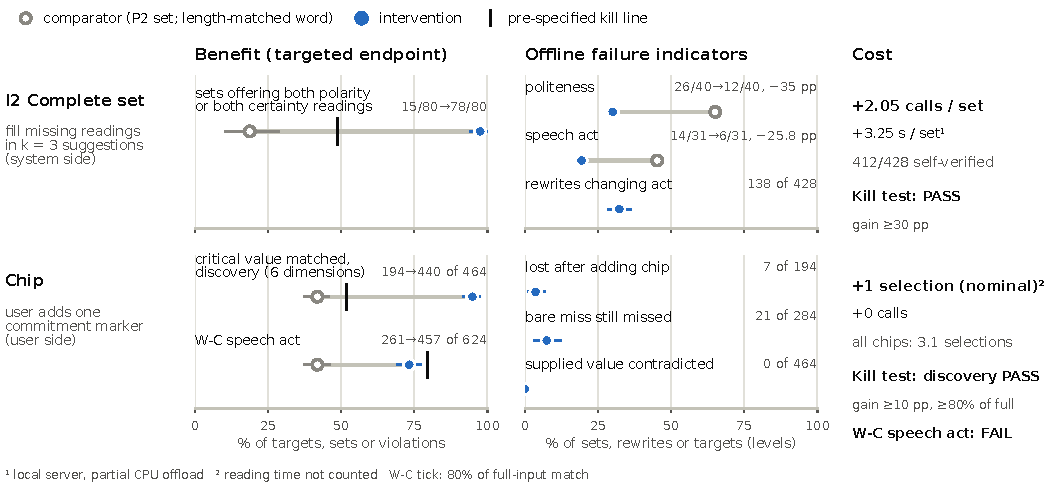
\includegraphics[width=\textwidth]{fig_ledger}
\caption{Two add-ons help in one place and cost something elsewhere (machine-extracted labels; four models).
Open circle: comparator; filled: intervention; bars: 95\% cluster-bootstrap intervals; black tick: the pass line set in advance; pp: percentage points.
Plotted values are percent \emph{levels}; changes in points are printed.
The cue passes both clauses on the development set but \emph{fails} its $\geq$80\%-of-typed clause on the confirmation set (only its gain clause replicates).
The guard is in Table~\ref{tab:guard}.}
\label{fig:ledger}
\end{figure*}

\subsection{The guard: about half of failures repaired, and feedback beats plain retrying}
On the development cue conditions, strict-check pass rose from \RES{g_spx_p0}\% to \RES{g_spx_g1}\% of \RES{n_cue_targets} targets (Table~\ref{tab:guard}).
Of the \RES{g_fixc_n} initial failures the guard repaired \RES{g_fixc_k} (\pci{g_fix}), far above its 30\% pass line.
Deleting an unrequested \say{please} at zero calls already reaches \RES{c3_guard_pass_g1s} strict-check passes, so regeneration's increment is \RES{c3_guard_increment} points [\RES{c3_guard_increment_lo}, \RES{c3_guard_increment_hi}]: \RES{c3_guard_g1_only} targets pass only with the guard and \RES{c3_guard_strip_only} only with deletion.
\RES{g_unfixed_k} of \RES{g_unfixed_n} failures remained, \RES{g_res_act_k} of them involving speech act, and \kof{g_res_flag} were still flagged after both retries: detected, not repaired.
\slotBaselineRes{} % BASELINE

\paragraph{Confirmation.}
Speech act was the guard's weakest dimension, so we reran the guard unchanged on the confirmation set's speech-act families (\RES{gt_fam} families, four models, three cue conditions, \RES{gt_targets} targets).
Criteria were frozen before any retry: at least 30\% of strict failures repaired, at most 10\% of strict-correct texts changed, and a joint-pass gain whose lower 95\% bound exceeds zero.
The pass rate rose from \RES{gt_jp_p0}\% to \RES{gt_jp_g1}\%, \RES{gt_jgain_g1} points [\RES{gt_jgain_g1_lo}, \RES{gt_jgain_g1_hi}]; the guard repaired \kof{gt_rep_g1} strict-check failures (\pci{gt_rep_g1}), changed \kof{gt_cc_g1} already-correct texts and turned \RES{gt_pf_g1_k} of the strict-check passes into failures.
Only the \RES{pf_chg_n} changed texts could have failed, so the informative figure is \RES{pf_chg_k} of \RES{pf_chg_n} (95\% upper bound \RES{pf_chg_ub}\%); the strict predicate shares lexical logic with the monitor and the guard returns its first unflagged attempt, so the zero is partly by construction.
The shown row 1 is not such a failure by the scorer's labels; a post hoc lexical rule finds a bracketed chip token in \kof{lk_chg} of the changed texts, \kof{lk_arm} of all guard strict-check passes and \kof{lk_p0} of first-pass passes, and a person is needed for malformed text of other kinds (Section~\ref{sec:repaircost}).
Every scored criterion passed within the call caps.
The gain is uneven across the four fixed models: +\RES{gt_jgain_terra} (API model), +\RES{gt_jgain_qwen} (Qwen), +\RES{gt_jgain_llama} (Llama) and +\RES{gt_jgain_gemma} points (Gemma), \RES{gt_jgain_gemma_n} targets each, so the pooled figure comes mostly from the two weaker models.
The labels behind every treated-output number were validated on untreated outputs only; no human relabelled guard-treated text beyond the \RES{p17_texts_rep} repaired texts of the audit below.
The repair rate fell from \RES{g_fix}\% (strict-check; \RES{gd_jrep}\% joint) in development to \RES{gt_rep_g1}\% (\RES{gw_jrep}\% joint) on fresh items, so the development figure overstates it; joint-pass and strict-check rates are not interchangeable.
Deletion alone gained \RES{gt_jgain_g1s} points, so the guard's increment over it is \RES{gt_cmp_joint} points [\RES{gt_cmp_joint_lo}, \RES{gt_cmp_joint_hi}], and \RES{gt_res_g1}\% of targets remain strict-check failures.
Of the results here, the guard's three frozen confirmation criteria are confirmatory; the resample baseline, the audit's secondary endpoints, H1 and H2, the decomposition and the frontier rows are post hoc or exploratory.

\subsection{What the pass does not show: repair usability}
\label{sec:repaircost}
A pass checks a few labels, not a sentence.
For \kw{\chip{ASK} \chip{YOU} \chip{PLAIN} wear headphones}, the guard turns \say{You wear headphones.} into \say{Ask you to wear headphones.}, which passes every scored predicate (Figure~\ref{fig:examples}).
The pattern is common: \RES{g_ask_k} of the \RES{g_ask_n} scored development repairs begin ``Ask you'' (post hoc lexical count).
We therefore had people judge repaired text.
\textbf{The audit.}
A \RES{p17_all}-text audit of new texts (\RES{p17_prim} primary: \RES{p17_texts_rep} repaired, \RES{p17_prim_ctl} never-failed controls; \RES{p17_sec} secondary: 20 original-failed and 20 strip-only texts, to separate repair from item difficulty) gave each text \RES{p17_raters} independent non-author raters, under a rule frozen before any return: a pooled interval entirely below $-$\RES{p17_margin} points kills the guard for deployment (kept as a detector); one including $-$\RES{p17_margin} but excluding 0 is a cost of uncertain size; one including 0 is no detectable cost.
\slotAuditBody{} % PART17

\subsection{Two more ledger rows: the menu and the cue}
The complete menu raises coverage of both polarity or certainty readings (+\RES{s_pc_dx} points, passes its line) but removes the polite option on other dimensions (Figure~\ref{fig:examples}, row 2).
The cue keeps the critical value in \RES{c_chip1}\% of development targets (\RES{c_ratio}\% of typed input), and its gain over the length-matched word replicates on \RES{wc_act_fam} fresh speech-act families (\RES{t4_wc_base} points [\RES{t4_wc_base_lo}, \RES{t4_wc_base_hi}]), but there it reaches \RES{wc_act_ratio}\% of the typed-input rate, below its 80\% line (Figure~\ref{fig:ledger}).
\slotLegend{} % LEGEND_TEST

\subsection{Realistic-input checks}
\label{sec:realistic}
We ran the pipeline on \RES{hw_kept} minimal pairs written by \RES{hw_writers} non-author annotators and on keywords that \RES{el_annot} annotators typed for \RES{el_msgs} AACText messages.
On the human-written pairs the cue gain replicates on all \RES{hw_chip_dims} dimensions (\RES{hw_chip_min} to \RES{hw_chip_max} points), and the three confirmation contrasts replicate in direction: speech-act cue +\RES{t6_p1} points, politeness addition +\RES{t6_p2}, and a bare affirmative default of \RES{hw_p3}\% \ci{hw_p3}.
Two controls on these pairs show that the missing cue, not the chip, is the lever.
An irrelevant chip from another dimension adds little: the cue chip beats it by \RES{cc_irrel_min} to \RES{cc_irrel_max} points by dimension.
On these pairs the same cue as a plain word (\kw{not}, \kw{please}) was declared equivalent to the chip (interval within $\pm$5 points) on \RES{cc_eq_n} of \RES{cc_nl_dims} dimensions (largest difference \RES{cc_eq_max}); the chip leads by under 1 point on polarity and time/quantity, and the word beats the chip on speech act by \RES{cc_nl_act} points.
With \RES{hw_wr_min}--\RES{hw_wr_max} writers per contrast we claim direction and consistency only: every writer's mean has the same sign, and the replication is exploratory.
In the keyword study about one keyword set in five lost the negation (\RES{el_pol_h}\% \ci{el_pol_h}; \RES{t2_d_h}\% [\RES{t2_d_h_lo}, \RES{t2_d_h_hi}] after resampling messages and reweighting to the sampling frame), on cue-enriched messages that carry a negation.

\paragraph{Defaults: a good guess with an asymmetric cost.}
When keywords carry no negation word, the models write an affirmative sentence for \RES{t2_aff_h}\% of such human keyword sets.
That is the Bayes-preferred guess: \RES{t2_neg_prev}\% of AACText messages are negated, and among human keyword sets with no negation word the source was negated only \RES{t2_post_h}\% [\RES{t2_post_h_lo}, \RES{t2_post_h_hi}] of the time (\RES{t2_post_h_bayes}\% from corpus prevalence), against \RES{t2_post_c}\% for the crude compressor; here $p$ is the probability that the typed source was negated given a keyword set with no negation word, whereas \RES{t2_neg_prev}\% is the unconditional share of negated messages, and Section~\ref{sec:frontier}'s \RES{fr_post}\% is the same $p$ on that analysis's \RES{fr_units} exposure units; guessing affirmative is right \RES{t2_acc_h}\% of the time.
The harm is the asymmetric cost: about \RES{t2_rev_h} [\RES{t2_rev_h_lo}, \RES{t2_rev_h_hi}] of every 1,000 messages are silently reversed when the user types keywords unaided (a posterior-based estimate from the keyword study; Table~\ref{tab:rev} lists it with the two other estimates of the same quantity), against \RES{t2_spur_h} spurious negations, and the guess breaks even only if a reversal costs under \RES{t2_ratio_h} times a spurious negation (the posterior odds $(1-p)/p$).
An accuracy metric rewards this behavior, so a ledger puts a default's cost beside its hit rate.
Four affirmative rates use different inputs and are not interchangeable: \RES{t2_aff_h}\% of human keyword sets with no negation word; \RES{hw_p3}\% of bare human-written pairs; \RES{lg_b}\% to \RES{lg_c}\% of committed answers on bare polarity inputs across the legend arms (four models, one greedy draw each; \RES{lg_c}\% when told not to assume).
The default holds on the \RES{mb_nmod} models from \RES{mb_nfam} families (at least \RES{mb_bare_min}\% affirmative) and on a lite Gemini model (\RES{mb_gem_a}\% and \RES{mb_gem_c}\% on the legend arms).
\citet{chen2023say} reported that models write sentences wrongly positive about negative commonsense facts in keyword-to-sentence generation; their measurements are on negative commonsense facts, not AAC messages; we price the default against a human base rate on AAC-style messages and show it survives \say{do not assume} prompting.

\subsection{Two ledger columns from people: writer intent and clinical weight}
\label{sec:human}
\paragraph{Writer intent (first test of H1).}
Each of \RES{p18_n_writers} writers judged \RES{p18_per_writer} outputs generated from their own pairs (\RES{p18_n_items} in all), choosing the version they meant.
A cue raises the share matching the intended version from \RES{p18_m_bare}\% to \RES{p18_m_cue}\%, +\RES{p18_cue} points [\RES{p18_cue_lo}, \RES{p18_cue_hi}] (writer-clustered; keywords-only is a reference level, not a failure rate).
Yet writers accepted \RES{p18_asis_k} of all \RES{p18_asis_n} outputs as written with no edit (a different test from naming the version they meant), and the judge's critical-dimension label agrees with the writer's four-way label at only $\kappa=\RES{p18_wj_kappa}$.
Keeping the critical commitment is necessary, not sufficient.
Among the \RES{p18_right_na_n} of those \RES{p18_asis_n} outputs whose critical value the judge scored correct (\RES{p18_right_r1_n} with a decided answer; \RES{p18_right_unsure} unsure), writers rejected \kof{p18_right_r1} as not the version meant.
A post hoc decomposition (exploratory; classifier agreement with \RES{wm_hand_n} hand-coded items $\kappa=\RES{wm_kappa}$, optimistic because its rules followed those items) finds mainly compression loss and event/role misresolution among the judge-correct outputs writers did not accept: \RES{p18_right_dropped}\% of the writers' sentences contain words no keyword supplied, \RES{p18_right_subst}\% of the outputs change who does what, and added content is the primary reason in \RES{p18_added_only} cases but is present in \RES{p18_right_added}\% of these outputs (the judge's added-content flag: \RES{p18_right_jadded}\%).
Two AAC-user design consultants independently asked that relations (who does what) be preserved.
\paragraph{Clinical weight.}
Two speech-language pathologists (expert review of study materials, not a population estimate) rated how serious each of seven kinds of silent meaning change is; both rated a dropped or added negation \RES{slp_neg_sev} of 5 and would block it.
Weighting each judge-flagged failure by the severity of its type, the guard lowers the clinically weighted failure rate from \RES{slp_wc_base}\% to \RES{slp_wc_guard}\% (confirmation) and a supplied cue lowers it on human-written pairs from \RES{slp_hw_base}\% to \RES{slp_hw_chip}\% (chip) and \RES{slp_hw_word}\% (word); on selected judge-failed items they judged repairs acceptable to speak in \kof{slp_acc_rep} rater-judgments against \kof{slp_acc_orig} for the originals (descriptive, not comparable arms).

\subsection{Frontier limits: the cue's measured price, and what asking and uncertainty do not do}
\label{sec:frontier}
These results are provisional: stored outputs, machine labels resolved by a blind arbiter, the three local primary models (Gemma-3-4B, Llama-3.1-8B, Qwen2.5-7B), \RES{fr_units} exposure units.
\begin{table}[t]
\centering\footnotesize
\setlength{\tabcolsep}{3pt}
\begin{tabular}{@{}>{\raggedright\arraybackslash}p{2.2cm}>{\raggedright\arraybackslash}p{3.4cm}>{\raggedright\arraybackslash}p{1.9cm}@{}}
\toprule
Estimator & Unit resampled & Silent reversals per 1,000\\
\midrule
Posterior (Sec.~\ref{sec:realistic}) & messages, reweighted to the sampling frame & \RES{t2_rev_h} [\RES{t2_rev_h_lo}, \RES{t2_rev_h_hi}]\\
Model-visible & exposure units & \RES{fr_ac} [\RES{fr_ac_lo}, \RES{fr_ac_hi}]\\
Bare-arm regeneration & same items, regenerated bare (point rate) & \RES{fr_pol_bare}\\
\bottomrule
\end{tabular}
\caption{Three estimators of one quantity, not independent replications.}
\label{tab:rev}
\end{table}
Always committing leaves about \RES{fr_ac} silent negation reversals per 1,000 messages by the model-visible estimator (Table~\ref{tab:rev}); the abstract and the cue comparison below use the bare-arm regeneration rate, \RES{fr_pol_bare}, because it shares items with the cue arms.
Supplying the cue on every message (derived: bare rate times the share not restored, regenerated on the same items) cuts polarity reversals per 1,000 from \RES{fr_pol_bare} [\RES{fr_pol_bare_lo}, \RES{fr_pol_bare_hi}] to \RES{fr_pol_chip} [\RES{fr_pol_chip_lo}, \RES{fr_pol_chip_hi}] (chip) and \RES{fr_pol_word} [\RES{fr_pol_word_lo}, \RES{fr_pol_word_hi}] (word), and politeness reversals from \RES{fr_pt_bare} to \RES{fr_pt_chip} and \RES{fr_pt_word}; the chip and the word are not distinguishable on polarity or speech act on these items; speech-act restoration is \RES{fr_sa_chip}\% with a chip and \RES{fr_sa_chipg1}\% with chip plus guard.
Ask policies, including a CLAM-style trigger (\RES{fr_clam} reversals per 1,000 against \RES{fr_rand} for gated random), show no detectable benefit over gated-random asking after Holm correction (power limited, not equivalence), and model sampling uncertainty ranks at-risk inputs at AUROC \RES{fr_auc_samp} against \RES{fr_auc_lex} for a lexical model.
The cue has to come from the user.

%% =====================================================================
\section{From Ledger to a Pre-Specified Human-Effect Study}
\label{sec:protocol}
%% =====================================================================
\begin{table}[t]
\centering\footnotesize
\setlength{\tabcolsep}{3pt}
\begin{tabular}{@{}>{\raggedright\arraybackslash}p{1.7cm}>{\raggedright\arraybackslash}p{5.8cm}@{}}
\toprule
\multicolumn{2}{@{}p{7.5cm}}{\textbf{H3 study: micro-randomized trial (MRT), pre-specified design; no value is a result}}\\
\midrule
Estimand & Average causal excursion effect~\cite{boruvka2018excursion} on a proximal outcome of delivering the regenerated sentence versus the original, at decision points where the monitor flags a conflict, for adult AAC users who compose with LLM keyword expansion\\
Arms, unit & Randomized per flagged message within user~\cite{klasnja2015mrt}, fixed probabilities: silent regeneration, flag-and-confirm, original; cues can only be offered, so they are a between-user factor\\
Outcomes & Proximal: sent without edit, one-tap \say{said what I meant} on a random subset of sends, time to send. Longitudinal: weekly rates, abandonment, reliance, week as moderator\\
Assumptions & Positivity (every flagged point has a nonzero chance of each arm, by design); consistency (the delivered sentence is the arm); no interference across a user's decision points beyond what we model; carryover is the main threat, so we target the excursion effect (deviate once, then resume usual practice)\\
Sample size & Illustrative, one two-arm between-user contrast with a cluster design effect, no multiplicity adjustment, typed assumptions to replace with pilot estimates: standardized effect \RES{mrt_d}, within-user correlation \RES{mrt_rho}, \RES{mrt_T} flagged points per user, 80\% power, 5\% level, about \RES{mrt_users} users. The monitor flagged about \RES{g_flagged}\% of constructed inputs (real-use rate unknown), so \RES{mrt_T} flagged points need roughly \RES{mrt_msgs} messages per user, a feasibility limit of its own\\
Analysis & Weighted, centered least squares with user-clustered errors\\
\bottomrule
\end{tabular}
\caption{The human-effect study that tests H3.}
\label{tab:mrt}
\end{table}
Each prediction names its test and what would demote it; H1 and H2 were checked post hoc on data already seen, and the H3 design is pre-specified in version control.

\paragraph{Predictions.}
\textbf{H1 (writer intent).} Among outputs the scorer counts as preserving a writer's critical value, writers report that the output \say{said what I meant} more often than among outputs it counts as failing; a gap whose interval includes zero demotes the scored endpoint.
\slotIntent{} % PART18
\textbf{H2 (repair usability).} A scored repair is usable at no less than \RES{p17_margin} points below a never-failed control; the \RES{p17_all}-text audit tested this under the frozen rule of Section~\ref{sec:repaircost}, so H2 is unresolved.
\textbf{H3 (collateral).} Offline changed-correct and coverage loss predict a later drop in users' \say{said what I meant} rate; if not, evaluation of this kind should be demoted.
H3 needs AAC users and is the MRT of Table~\ref{tab:mrt}.

\paragraph{Design implications from two AAC-user consultants.}
Two paid AAC-user design consultants rated our five requirements (keep a button's meaning; do not change typed text; do not quietly guess; a new button must not break what was right; an honest test screen) important, and each asked for a sixth (we report requirement changes only): \textbf{R6, a draft is never spoken without the person's approval}, with the original words kept beside the draft and speaking a separate deliberate act.
They also asked for an exact-copy default for typed sentences, a visible scope for NOT, and showing where two drafts differ; R6 makes flag-and-confirm the default design.

%% =====================================================================
\section{Limitations}
\label{sec:limits}
%% =====================================================================
\emph{Human outcomes and raters.} Results are changes in stored text; communication success, agency, effort and trust are untested (Section~\ref{sec:protocol}), and the audit's raters are non-author peers, not AAC users.
\emph{Labels and scope.} Endpoints use an LLM extractor validated on untreated outputs only, with post-outcome arbitration in the confirmation; strip-only covers one failure type; the menu was not run on the confirmation set; items are constructed, open models are at most 14B and 4-bit, and AACText is crowd-written fiction.
\emph{Community involvement.} Two paid AAC-user design consultants and two speech-language pathologists reviewed requirements and study materials (n=2 each; expert review, not a population estimate); the requirements remain our proposals, with no claim of benefit to AAC users.
\emph{Ethics.} No data were collected from AAC users.
All annotators were adult non-authors recruited from the authors' university peers, identified only by an ID; each consented and was reimbursed for their time. They labelled model outputs and audited items under a fixed codebook, blinded to model, condition and source; some also chose keywords for public AACText messages or wrote new sentence pairs, released under CC~BY~4.0 with recorded consent. No personal or health data were collected, and we did not seek an institutional review determination.

\section{Conclusion}
On the confirmation set's speech-act families the guard raises the joint pass rate by +\RES{gt_jgain_g1} points, repairs \RES{gt_rep_g1}\% of strict-check failures with \RES{pf_chg_k} of \RES{pf_chg_n} changed texts failing, and beats resampling at matched temperature (+\RES{bw_tr} points).
In the human audit, repairs keep the meaning and remove invented stance relative to their failed originals in an exploratory paired contrast on \RES{p17_pres_pairs} pairs, though they are not more usable than those originals; against never-failed controls the frozen rule returns no detectable cost, the deployment clause is unresolved and stricter endpoints show a cost (Section~\ref{sec:repaircost}).
A supplied cue removes nearly all silent reversals on the same items.
The ledger records what remains (deletion alone earns +\RES{gt_jgain_g1s} of the +\RES{gt_jgain_g1} points; writers accept \RES{p18_asis_k} of \RES{p18_asis_n} outputs as written), and the pre-specified study turns these into predictions that AAC users can test.
Scripts that rebuild every number accompany this submission. % VERIFY: attach the anonymized archive before submission

%% GenAI disclosure: the lab supplies the format (placeholder).

\bibliography{refs}

\end{document}
